\documentclass[preprint,12pt]{elsarticle}

\usepackage{amsmath,amssymb,amsthm}
\usepackage{graphicx}
\usepackage{booktabs}
\usepackage{makecell}
\usepackage{rotating}
\usepackage[hidelinks]{hyperref}
\usepackage{lineno}
\usepackage{xcolor}
\usepackage{microtype}
\usepackage[section]{placeins}
\setlength{\emergencystretch}{2em}

\newtheorem{proposition}{Proposition}
\newtheorem{theorem}{Theorem}
\newcommand{\appref}[1]{\ref{#1}}
\makeatletter
\newcommand{\inputtable}[1]{\@@input #1 }
\makeatother
\journal{Sustainable Operations and Computers}

\begin{document}

\begin{frontmatter}

\title{Anticipating demand in carbon-aware scheduling across data centers: guarantees and fair carbon attribution\tnoteref{abbr}}
\tnotetext[abbr]{Abbreviations: ACI, adaptive conformal inference; ASAP, as soon as possible; CARMA, Carbon-aware Anticipatory Receding-horizon Multi-site Allocation; EDF, earliest deadline first; EIA, U.S. Energy Information Administration; GB, Great Britain; GBM, gradient-boosted model; HAC, heteroskedasticity- and autocorrelation-consistent; IR, individual rationality; MAE, mean absolute error; MEF, marginal emission factor; MPC, model predictive control; NESO, National Energy System Operator; ONS, Operador Nacional do Sistema El\'etrico; PUE, power usage effectiveness; RMSE, root mean squared error.}

\author{Quang-Vinh Dang\corref{cor1}}
\ead{vinh.dq4@buv.edu.vn}
\cortext[cor1]{Corresponding author. ORCID: 0000-0002-3877-8024}
% TODO before submission: add the street address and postcode of the affiliation (Guide for Authors: full postal address)
\affiliation{organization={British University Vietnam},
            city={Hung Yen},
            country={Vietnam}}

\begin{abstract}
Shifting deferrable jobs to cleaner times and places cuts data-center emissions, but online schedulers act before future grid conditions and jobs are known. We formulate multi-site, deadline-constrained scheduling of bag-of-tasks jobs as a minimum-cost flow problem and study CARMA (Carbon-aware Anticipatory Receding-horizon Multi-site Allocation), which adds ``ghost jobs'' for expected arrivals to each hourly plan. Uncertainty about demand alone forces any online algorithm, even with perfect carbon forecasts, to a competitive ratio of $\Omega(\sqrt{\theta})$, where $\theta$ is the ratio of highest to lowest unit emission cost. Under explicit assumptions (a backstop resource, episodes within the planning window), CARMA never misses a deadline and is optimal under exact predictions; these assumptions do not hold in the weekly experiments. On 2024 regional grid data for Great Britain, CARMA comes within 8.0--9.8\% of the clairvoyant optimum, against 15.5--16.3\% for the best baseline without demand information. On four further fleets covering Europe, North and South America and Oceania, its gap is 2.7--5.8\% against 4.4--13.0\%. A scenario-based stochastic lookahead with the same demand information is level with CARMA or at most 1 point better, but needs 12--37 times more computing time. A trace-derived workload with a biased demand profile gives 21.2\% against 27.5\%. Under a stylized marginal-emission proxy, however, achievable reductions shrink to 14\% and CARMA's edge becomes small. Dual prices of the pooled problem give a carbon attribution in the core of the hindsight pooling game, whereas origin- and host-based accounting violate coalitional stability in every week.
\end{abstract}

\begin{keyword}
Carbon-aware computing \sep Data center scheduling \sep Competitive analysis \sep Minimum-cost flow \sep Cooperative cost allocation \sep Carbon intensity forecasting
\end{keyword}

\end{frontmatter}

\linenumbers

\section{Introduction}\label{sec:intro}

Data centers are among the fastest-growing electricity consumers. Efficiency gains kept their energy use nearly flat through the 2010s even as computing output grew several-fold~\cite{masanet2020recalibrating,shehabi2016united}. That buffer is now thinning, and information and communication technology accounts for an estimated 2.1--3.9\% of global greenhouse-gas emissions~\cite{freitag2021real}. Large machine-learning workloads have drawn particular attention~\cite{strubell2019energy,patterson2022carbon,dodge2022measuring}. The carbon intensity of grid electricity varies by a factor of ten or more across regions and hours, driven by the output of wind, solar and dispatchable plant~\cite{staffell2017measuring}. Operators can therefore cut emissions without new hardware by moving flexible work to cleaner places and times. Such \emph{carbon-aware computing}~\cite{radovanovic2023carbon,bashir2021enabling} is an operations problem: capacity is finite, deadlines bind, and both the grid and the job stream are uncertain.

Batch jobs such as model training, analytics, rendering and backups are a natural target, because they tolerate some delay. Previous work has shown the potential of temporal shifting (running later)~\cite{wiesner2021lets,goiri2012greenhadoop,hanafy2023carbonscaler} and of spatial shifting (running elsewhere)~\cite{liu2011greening,zheng2020mitigating}. It has also shown their limits. Sukprasert et al.~\cite{sukprasert2024limitations} found that practical reductions from spatio-temporal shifting fall well short of idealized bounds. Most methods are evaluated with a scheduler that reacts to the jobs it has already seen, using point forecasts of carbon intensity. Three questions have received less attention. First, how much is lost because an online scheduler does not know which jobs will arrive next, and can any scheduler guarantee good performance in the worst case? Second, does it pay to price the uncertainty of carbon-intensity forecasts into scheduling decisions? Third, when several sites pool their capacity, how should the resulting emissions be attributed so that every participant is better off than on its own?

This paper addresses these questions with a scheduling policy, guarantees under explicitly stated assumptions, and a controlled evaluation on three years of hourly grid data for Great Britain, Europe, the United States, Brazil and New Zealand. Its building blocks (receding-horizon planning, network flows, conformal calibration and dual cost allocation) are standard; the contribution lies in their combination for this problem, the lower bound, the conditions under which the guarantees hold and the empirical evidence. It makes five contributions.
\begin{enumerate}
\item \textbf{Formulation.} We state multi-site, deadline-constrained, width-limited scheduling of deferrable bag-of-tasks jobs, including the emissions of data transfer, as a minimum-cost flow problem (Proposition~\ref{prop:flow}). Offline clairvoyant optima and every online planning step can therefore be solved to optimality, after quantization, by fast combinatorial min-cost flow algorithms. We also prove that myopic receding-horizon scheduling can be arbitrarily worse than the clairvoyant optimum even with perfect carbon forecasts (Proposition~\ref{prop:myopic}).
\item \textbf{Algorithm.} We propose CARMA (Carbon-aware Anticipatory Receding-horizon Multi-site Allocation). At every hour, CARMA adds \emph{ghost jobs} to its planning network. These represent expected arrivals, learned from the operator's history, so the planner reserves scarce low-carbon capacity for work that has not yet arrived. The planning problem stays a single min-cost flow and decisions take tens of milliseconds.
\item \textbf{Guarantees.} We prove that uncertainty about demand alone forces every online algorithm, even one with perfect carbon forecasts, to a competitive ratio of $\Omega(\sqrt{\theta})$, about $\sqrt{\theta}/2$ for large $\theta$, where $\theta$ is the ratio of the highest to the lowest unit emission (Theorem~\ref{thm:lb}). In an idealized setting with a backstop resource, CARMA never misses a deadline whatever its predictions, so it inherits the $\theta$-competitiveness that every on-time policy has. If, in addition, each episode fits within the planning window, CARMA is optimal when its predictions of demand and carbon are exact, and its excess emissions grow at most linearly in the prediction errors (Proposition~\ref{prop:robust} and Theorem~\ref{thm:carma}). These assumptions do not hold in our weekly experiments, so we verify the theorem separately in episodes that satisfy them. We also show that the dual prices of the pooled scheduling network give a carbon attribution among sites that lies in the core of the pooling game, so no group of sites gains by leaving (Theorem~\ref{thm:core}).
\item \textbf{Forecasting and recalibration pipeline.} As a tool for the scheduling study, we build a reproducible 1--24-hour carbon-intensity forecaster from a public feed: direct gradient-boosted models with horizon-wise normalized conformal quantiles and adaptive recalibration, which keeps empirical coverage close to target under the decarbonization drift of 2024. Its quantiles let us test risk-adjusted carbon pricing inside the scheduler. We do not claim a new forecasting method.
\item \textbf{Evidence design.} We evaluate CARMA out of sample on 52 weeks of 2024, with three workload traces per week, three load levels and two operating regimes. We add a trace-derived workload from the Alibaba 2018 cluster trace and four further fleets built from open generation data for Europe, the United States, Brazil and New Zealand. CARMA is compared with seven implementable online baselines, including a revenue-management protection-level policy and a scenario-based stochastic lookahead that uses the same demand information, with clairvoyant and ablated variants, and with the clairvoyant oracle. The experiments separate the value of anticipating demand from the value of better carbon forecasts, characterize how performance degrades with prediction errors, test the conclusions under a stylized marginal-emission accounting, and assess the stability of origin-based, host-based, Shapley and dual carbon attribution.
\end{enumerate}

The emission figures in this paper are attributional, based on average grid intensities, and Section~\ref{sec:sens} examines how they change under a stylized marginal-emission accounting. The rest of the paper is organized as follows. Section~\ref{sec:related} reviews related work. Section~\ref{sec:methods} presents the model, the forecaster, CARMA and the experimental design. Section~\ref{sec:theory} establishes the theoretical guarantees, with proofs in \appref{app:proofs}. Section~\ref{sec:results} reports results, Section~\ref{sec:discussion} discusses implications and limitations, and Section~\ref{sec:conclusion} concludes.

\section{Related work}\label{sec:related}

\paragraph{Carbon-aware workload shifting} Early green data-center schedulers matched deferrable jobs to on-site solar production, for example GreenSlot~\cite{goiri2011greenslot} and GreenHadoop~\cite{goiri2012greenhadoop}. Other work exploited electricity-price and carbon differences across sites through geographical load balancing~\cite{rao2010minimizing,liu2011greening} and dynamic right-sizing~\cite{lin2013dynamic}. With public carbon-intensity feeds, attention moved to grid emissions. Wiesner et al.~\cite{wiesner2021lets} quantified the reductions from temporal shifting in several regions, including Great Britain, and proposed forecast-based lowest-window scheduling. Google's carbon-intelligent compute system sets next-day virtual capacity curves from carbon forecasts and forecasts of the fleet's own demand~\cite{radovanovic2023carbon}. It is the closest industrial precedent for using demand forecasts, but it shapes hourly virtual capacity curves per cluster rather than planning individual jobs across sites. Cucumber admits delay-tolerant work only when forecast renewable supply allows it~\cite{wiesner2022cucumber}, and Caribou shifts serverless functions between regions~\cite{gsteiger2024caribou}. CarbonScaler varies the allocation of elastic jobs with carbon intensity~\cite{hanafy2023carbonscaler}. Ecovisor exposes the energy system to applications~\cite{souza2023ecovisor}. Carbon Explorer weighs scheduling against investment in renewables and storage~\cite{acun2023carbon}. Load migration between data centers can absorb curtailed renewable generation~\cite{zheng2020mitigating}, and data-center demand response has been surveyed in~\cite{wierman2014opportunities}. Sukprasert et al.~\cite{sukprasert2024limitations} bound the potential of spatio-temporal shifting across 123 regions and find that simple policies capture most of the achievable benefit. Our study complements theirs by identifying \emph{which} information limits online schedulers when capacity at clean sites is scarce.

\paragraph{Online algorithms and guarantees} Worst-case analysis of carbon-aware scheduling builds on online search and one-way trading~\cite{elyaniv2001optimal}, for which threshold policies achieve optimal competitive ratios. Lechowicz et al.\ derived optimal double-threshold algorithms for the online pause-and-resume problem~\cite{lechowicz2023online}. With CarbonClipper, they also derived learning-augmented algorithms with an optimal consistency--robustness trade-off for spatiotemporal allocation of a single deadline-constrained workload over a network of data centers~\cite{lechowicz2025learning}. These works model uncertainty about future carbon \emph{prices} for one job. We study many jobs that compete for finite low-carbon capacity, and we show that uncertainty about \emph{demand} creates a distinct lower bound that carbon forecasts cannot remove. Our guarantees follow the consistency--robustness paradigm of algorithms with predictions~\cite{lykouris2021competitive}. CARMA's re-solving of a deterministic plan with expected future demand is an instance of the certainty-equivalent re-solving heuristics of network revenue management~\cite{jasin2012resolving}. Our contribution is not the device itself but its formulation as a single flow problem for carbon-aware scheduling, the guarantees and the empirical attribution of value. Table~\ref{tab:related} positions the closest work along the dimensions that matter here.

\begin{table}[!htbp]
\centering
\caption{Positioning against the closest work, as modeled in the cited studies ($\checkmark$: explicitly modeled or provided; --: not modeled).}
\label{tab:related}
\footnotesize
\footnotesize\setlength{\tabcolsep}{3pt}
\begin{tabular}{p{4.3cm}cccc}
\toprule
Work & \makecell{Many jobs share\\finite capacity} & \makecell{Information on\\future demand} & \makecell{Worst-case\\guarantee} & \makecell{Attribution\\among sites} \\
\midrule
Lowest-window temporal shifting~\cite{wiesner2021lets} & -- & -- & -- & -- \\
Geographical load balancing~\cite{liu2011greening} & $\checkmark$ & -- & -- & -- \\
Carbon-intelligent compute system~\cite{radovanovic2023carbon} & $\checkmark$ & $\checkmark$ & -- & -- \\
Online pause-and-resume~\cite{lechowicz2023online} & -- & -- & $\checkmark$ & -- \\
CarbonClipper~\cite{lechowicz2025learning} & -- & -- & $\checkmark$ & -- \\
Flow models of preemptive scheduling~\cite{horn1974some,federgruen1986preemptive} & $\checkmark$ (offline) & -- & -- & -- \\
This paper & $\checkmark$ & $\checkmark$ & $\checkmark$ (A1--A2) & $\checkmark$ \\
\bottomrule
\end{tabular}
\end{table} Our fairness result draws on cooperative game theory: linear production games and flow games have non-empty cores that can be computed from dual prices~\cite{owen1975core,kalai1982totally}.

\paragraph{Energy-aware scheduling in operations} Energy-efficient scheduling is a mature topic in manufacturing operations~\cite{gahm2016energy}, and green scheduling models have appeared in this journal, for example for parallel machines with job splitting~\cite{asadpour2022green} and for cloud resource allocation~\cite{sharma2024efficient}. Most such models are deterministic and solved offline, often with metaheuristics. We instead exploit exact network-flow structure and embed it in an online lookahead policy. Network-flow formulations of preemptive scheduling with release dates and deadlines go back to Horn~\cite{horn1974some} and Federgruen and Groenevelt~\cite{federgruen1986preemptive}. Proposition~\ref{prop:flow} extends this classical construction to multiple sites, job widths, time-varying emission costs and transfer emissions~\cite{ahuja1993network,orlin1997polynomial}. In the taxonomy of Powell~\cite{powell2019unified}, CARMA is a deterministic lookahead policy with a modified (anticipatory) model, in the spirit of model predictive control~\cite{rawlings2017model,mayne2000constrained}.

\paragraph{Carbon-intensity forecasting} Forecasts of grid carbon intensity use statistical decomposition~\cite{bokde2021short}, machine learning with many exogenous drivers~\cite{leerbeck2020short}, day-ahead regression for building demand response~\cite{lowry2018day}, and hierarchical models of the generation mix, as in CarbonCast~\cite{maji2022carboncast}. For Great Britain, NESO publishes regional forecasts through its Carbon Intensity API~\cite{nesoapi}. These are average (attributional) intensities. Marginal emission factors, which describe the plant that responds to a change in load, can differ substantially from averages and are the relevant measure for the system-level effect of load shifting~\cite{hawkes2010estimating,silerevans2012marginal}. These studies focus on point accuracy. For decisions, calibrated uncertainty matters as well. Conformal prediction~\cite{vovk2005algorithmic,lei2018distribution,angelopoulos2023conformal} provides distribution-free intervals and has been extended to quantile regression~\cite{romano2019conformalized}, to multi-horizon~\cite{stankeviciute2021conformal} and dynamic time series~\cite{xu2023conformal}, and to arbitrary distribution shift through adaptive conformal inference~\cite{gibbs2021adaptive}. We use these tools to build a recalibrated forecaster and to test, in a controlled way, whether risk-adjusted carbon costs improve scheduling. The question is motivated by the optimizer's curse~\cite{smith2006optimizer} and by the robust-optimization view that point-estimate solutions can be fragile~\cite{bental2000robust,bertsimas2004price}.

\section{Material and methods}\label{sec:methods}

\subsection{Problem setting}\label{sec:problem}

We consider an operator that runs a set $\mathcal{S}$ of data-center sites connected by a wide-area network. Time is divided into hourly slots $t=0,1,2,\dots$ Deferrable batch jobs arrive online. Job $j$ is released at the start of hour $a_j$ at origin site $o_j\in\mathcal{S}$. It carries $w_j$ server-hours of work made of independent tasks (a bag of tasks), can use at most $m_j$ servers concurrently, and must finish before the start of hour $d_j>a_j$. Work may be paused and resumed, and any part of it may run at a site other than its origin. Remote execution requires moving input data. At site $s$ and hour $t$, $K_s(t)$ servers are free for batch work once the interactive load has been served.

Let $I_s(t)$ be the average carbon intensity of the electricity supplied to site $s$ during hour $t$ (gCO$_2$/kWh). Executing one server-hour of job $j$ at site $s$ during hour $t$ emits
\begin{equation}\label{eq:unitcost}
c_{o_j s}(t) = e\,\mathrm{PUE}_s\, I_s(t) + \mathbf{1}[s\neq o_j]\,\delta\,\eta\,\tfrac{1}{2}\big(I_{o_j}(t)+I_s(t)\big),
\end{equation}
where $e$ is the IT energy per server-hour, $\mathrm{PUE}_s$ is the power usage effectiveness of site $s$, $\delta$ is the data volume moved per migrated server-hour and $\eta$ is the energy intensity of network transfer (kWh/GB). The transfer term charges network energy at the mean intensity of the two endpoints. With decision variables $x_{js}(t)\ge 0$ (server-hours of job $j$ run at site $s$ in hour $t$), the offline version of the problem is the linear program
\begin{align}
\min_{x,u\ge 0}\quad & \sum_j\sum_{s}\sum_{t=a_j}^{d_j-1} c_{o_j s}(t)\,x_{js}(t) + \sum_j \Pi\, u_j \label{eq:obj}\\
\text{s.t.}\quad & \textstyle\sum_{s}\sum_{t=a_j}^{d_j-1} x_{js}(t) + u_j = w_j && \forall j, \label{eq:work}\\
& \textstyle\sum_{s} x_{js}(t) \le m_j && \forall j,\ t\in[a_j,d_j), \label{eq:width}\\
& \textstyle\sum_{j:\,a_j\le t<d_j} x_{js}(t) \le K_s(t) && \forall s,t, \label{eq:cap}
\end{align}
where $u_j$ is work left unfinished at the deadline and $\Pi$ is a lateness penalty much larger than any emission cost. When migration is not allowed, $x_{js}(t)=0$ for $s\neq o_j$; these variables are removed from the problem. With complete knowledge of arrivals and intensities, the optimum of (\ref{eq:obj})--(\ref{eq:cap}) is a lower bound on the emissions of every schedule that serves all jobs by their deadlines, and we use it as the \emph{clairvoyant oracle}. When emissions are evaluated only for a subset of jobs (Section~\ref{sec:data}), the oracle still has to serve every job under the same constraints but is charged emissions only for the evaluated ones, so that it remains a lower bound on the evaluated emissions of any schedule that meets all deadlines. Online policies that finish some work late lie outside this set; Section~\ref{sec:data} explains how we compare them. An online scheduler has to fix $x_{\cdot s}(t)$ at the start of hour $t$. At that point it knows the jobs released so far, the current intensities $I_s(t)$ and nothing more than forecasts of $I_s(t+h)$ and of future arrivals.

\begin{proposition}[Network-flow structure]\label{prop:flow}
Problem (\ref{eq:obj})--(\ref{eq:cap}) is a minimum-cost flow problem on a network with a source, one node per job, one node per (job, hour) pair, one node per (hour, site) pair and a sink. The source supplies $\sum_jw_j$ units of flow and the sink absorbs them. Arc capacities are $w_j$ (source$\to j$), $m_j$ ($j\to(j,t)$) and $K_s(t)$ ($(t,s)\to$ sink). The only arcs with a cost are $(j,t)\to(t,s)$, priced at $c_{o_j s}(t)$, and a slack arc $j\to$ sink priced at $\Pi$.
\end{proposition}
\begin{proof}
Because the supply equals $\sum_jw_j$ and arc source$\to j$ has capacity $w_j$, every such arc is saturated, and conservation at the job node is Eq.~(\ref{eq:work}). The capacity of arc $j\to(j,t)$ is Eq.~(\ref{eq:width}), conservation at $(j,t)$ splits that hour's work across sites, and the capacity of $(t,s)\to$ sink is Eq.~(\ref{eq:cap}). Conversely, every feasible flow defines a feasible $(x,u)$ with the same cost. The constraint matrix of the flow formulation is a node-arc incidence matrix, in which every column has exactly one $+1$ and one $-1$, so it is totally unimodular.
\end{proof}

Proposition~\ref{prop:flow} has a practical consequence. The oracle and every planning problem solved online (Section~\ref{sec:carma}) can be solved by combinatorial min-cost flow algorithms~\cite{ahuja1993network}, which return integral optimal flows for integral data. We quantize work, widths and capacities to $0.01$ server-hours (widths rounded up, capacities down) and costs to $0.01$~gCO$_2$, and solve the quantized network to optimality with the min-cost flow solver of OR-Tools~\cite{ortools} (version 9.15, a cost-scaling push-relabel algorithm). The solutions are therefore optimal for the quantized problem, and the simulator treats remaining work below 0.05 server-hours as complete; it checks every executed allocation against the capacity and width limits up to this tolerance. On the weekly clairvoyant problems (1{,}100--2{,}800 jobs), the flow solver returned the same objective as the LP solver HiGHS on the unquantized problem to within a relative $5\times10^{-5}$ and was 1.4--3.5 times faster (median 2.3; 0.3--1.2~s against 0.4--3.8~s; script \texttt{bench\_solvers.py}; one CPU core). The flow time includes two solves, for the emissions oracle and for the service-adjusted oracle, whereas the LP time is for one solve.

\subsection{Probabilistic carbon-intensity forecasting}\label{sec:forecast}

\paragraph{Point model} For each horizon $h=1,\dots,H$ ($H=24$ h) we fit a direct gradient-boosted regression tree model~\cite{friedman2001greedy} that predicts the change $I_s(t+h)-I_s(t)$ from information available at issue time $t$. Direct per-horizon models avoid the error accumulation of recursive strategies~\cite{taieb2012review}. One model per horizon is pooled across sites, with the site as a categorical feature. The features are the current intensity; differences between the current value and lags of 1, 2, 3, 6, 12 and 23 hours; the value observed at the same hour of the target on the previous day and in the previous week; a 24-hour rolling mean and mean absolute change (volatility); the national (GB) intensity; the regional wind, solar and gas shares; and calendar encodings of the target time (hour of day, day of week, annual sine and cosine). Models are fitted with absolute-error loss, so they estimate the conditional median. We use scikit-learn's histogram gradient boosting~\cite{pedregosa2011scikit} with 400 iterations, learning rate 0.05, 31 leaves and at least 50 samples per leaf. The models use only information available when the forecast is issued (gaps in the data are filled causally; Section~\ref{sec:data}), and no weather forecasts. This is deliberate: the goal is a forecaster any operator can build from a public intensity feed.

\paragraph{Conformal upper quantiles} A point forecast $\hat I_s(t+h\,|\,t)$ is turned into calibrated upper quantiles by split conformal prediction~\cite{vovk2005algorithmic,lei2018distribution} with normalized scores. On a calibration window disjoint from training, we compute for each site $s$ and horizon $h$
\begin{equation}
r_{s,h}(t) = \frac{I_s(t+h)-\hat I_s(t+h\,|\,t)}{\sigma_s(t)+\epsilon},
\end{equation}
where $\sigma_s(t)$ is the 24-hour mean absolute hourly change observed at issue time and $\epsilon=5$~gCO$_2$/kWh. Only pairs whose target $t+h$ also lies in the calibration window are used, so that no calibration outcome falls in the tuning period. For a target level $\beta$, the upper forecast is $U^{\beta}_s(t+h\,|\,t)=\hat I_s(t+h\,|\,t)+\hat q_{s,h}(\beta_{s,h}(t))\,(\sigma_s(t)+\epsilon)$, where $\hat q_{s,h}(\beta)$ is the $\lceil(n+1)\beta\rceil$-th smallest of the $n$ calibration scores, the split-conformal quantile. Grid carbon intensity is not exchangeable over time: 2024 was markedly cleaner than 2022--2023 (Fig.~\ref{fig:data}). We therefore update the working level online by adaptive conformal inference (ACI)~\cite{gibbs2021adaptive}. Once $I_s(t+h)$ is observed,
\begin{equation}\label{eq:aci}
\alpha_{s,h} \leftarrow \alpha_{s,h} + \gamma\big((1-\beta) - \mathbf{1}[I_s(t+h) > U^{\beta}_s(t+h\,|\,t)]\big),\qquad \beta_{s,h}(t)=1-\alpha_{s,h},
\end{equation}
with step size $\gamma=0.005$. At every hour, the outcomes observed in that hour update the levels before the new forecasts are issued, so feedback for horizon $h$ arrives $h$ hours after the forecast. When the working level reaches 1, the bound is set to the largest intensity of the site in the training period, a finite worst case in place of the infinite interval of ACI; when it reaches 0 the bound is zero, and bounds are floored at zero. Gap-filled outcomes give no feedback. For immediate feedback and unbounded intervals, ACI guarantees that the long-run miscoverage frequency converges to $1-\beta$ for any data sequence~\cite{gibbs2021adaptive}. Our variant has delayed feedback, a finite ceiling and a quantile grid of step 0.001, so we do not claim this guarantee and use ACI as an adaptive recalibration whose coverage is checked empirically (\appref{app:forecast}). The level $\beta$ then acts as a risk dial that remains roughly calibrated under drift, and with $\beta=0.5$ the procedure removes level shifts in the point model (a recalibrated median).

\subsection{CARMA: carbon-aware anticipatory receding-horizon multi-site allocation}\label{sec:carma}

A standard receding-horizon (model predictive control, MPC) scheduler~\cite{rawlings2017model} solves, at every hour $t$, the flow problem of Proposition~\ref{prop:flow} restricted to pending jobs and the window $[t,t+H)$. Future intensities are replaced by forecasts, and only the first hour of the plan is executed. Such a planner is \emph{myopic about demand}: it sees only jobs that have already arrived. The next result shows that this can be arbitrarily costly even when carbon intensities are known exactly.

\begin{proposition}[Myopia can be unboundedly costly]\label{prop:myopic}
Even with perfect intensity forecasts, myopic receding-horizon scheduling has no finite competitive ratio with respect to the clairvoyant oracle.
\end{proposition}
\begin{proof}
Take a clean site $A$ with one server and a dirty site $B$ with ample capacity. Let $c_A(0)=\varepsilon$, $c_A(1)=0$ and $c_B(0)=c_B(1)=c$, and ignore transfer costs. A flexible job ($w=1$, $m=1$) arrives at $t=0$ with deadline $d=2$. An urgent job ($w=1$) arrives at $t=1$ with $d=2$. At $t=0$ the myopic planner sees only the flexible job and defers it to $A$ at $t=1$ (cost $0<\varepsilon$). At $t=1$ both jobs must run in the same hour, one of them at $B$, so the total cost is $c$. The oracle runs the flexible job at $t=0$ and the urgent job at $t=1$, both at $A$, for a total of $\varepsilon$. The ratio $c/\varepsilon$ is unbounded as $\varepsilon\to 0$.
\end{proof}

The mechanism in Proposition~\ref{prop:myopic} is common in practice. Low-carbon capacity is scarce, and a myopic planner spends it on flexible work that could have waited or run elsewhere, leaving urgent jobs that arrive later to run on carbon-intensive capacity. CARMA addresses it by anticipating demand inside the same flow problem, and optionally prices forecast risk.

\begin{figure}[!htbp]
\centering
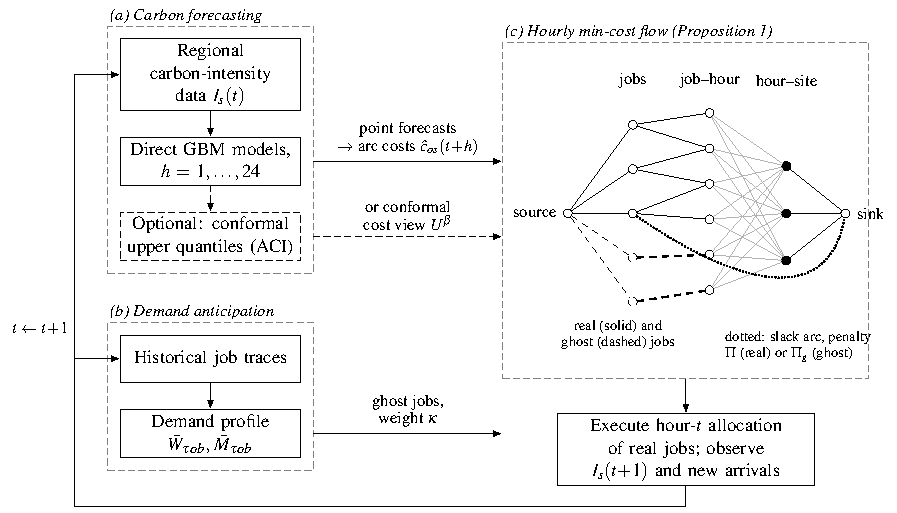
\includegraphics[width=\textwidth]{fig1_carma.pdf}
\caption{The CARMA decision loop. (a) Carbon-intensity forecasts price the job--hour to hour--site arcs; the selected configuration uses point forecasts, and conformal upper quantiles are an optional cost view. (b) A demand profile learned from past traces generates ghost jobs for expected arrivals. (c) Real jobs (solid) and ghost jobs (dashed) share one min-cost flow network, whose dotted slack arc carries unfinished work to the sink at the lateness penalty. The network is solved exactly every hour, and only the first-hour allocation of real jobs is executed.}
\label{fig:carma}
\end{figure}

\paragraph{Anticipated demand (ghost jobs)} From the operator's own history we estimate, for every hour of the week $\tau$, origin $o$ and window class $b$, the expected work $\bar W_{\tau ob}$ and the expected total width $\bar M_{\tau ob}$ of arriving jobs. Window classes are the bins $\mathcal{B}=\{1,2,4,6,9,13,18,24\}$ hours. A job is assigned to the largest bin not exceeding its window, so ghost jobs are never more flexible than the jobs they represent. Because binning shortens windows, the width of each ghost job is raised where necessary to at least its work divided by its window, which makes every ghost job window-feasible. At hour $t$, for each $k=1,\dots,\ell$ (the look-ahead), CARMA adds to the planning problem a \emph{ghost job} for every $(o,b)$ with work $\kappa\bar W_{\tau(t+k)ob}$, width $\kappa\bar M_{\tau(t+k)ob}$, release $t+k$ and deadline $\min(t+k+b,\,t+H)$. Ghost jobs compete with real jobs for capacity, but their slack arc is priced at a moderate penalty $\Pi_g$, set to $1.5$ times the largest local unit cost in the window, rather than at $\Pi$. They can therefore reserve clean capacity when it is economical but never force real work to be late. The weight $\kappa\ge 0$ scales how much of the expected demand is anticipated. With $\kappa=0$, CARMA reduces to myopic MPC.

\paragraph{Carbon cost view} Future-hour costs in Eq.~(\ref{eq:unitcost}) are evaluated at a forecast of $I_s(t+h)$; for the current hour ($h=0$) the observed intensity is used. CARMA admits two cost views: the point forecast $\hat I$, or the conformal upper quantile $U^{\beta}$ of Section~\ref{sec:forecast}. The second is motivated by the optimizer's curse~\cite{smith2006optimizer}: selecting the minimum over noisy estimates is biased toward optimism. The conformal view replaces each future cost by a calibrated quantile, which shifts it by a site- and horizon-specific amount proportional to the local volatility. For $\beta>0.5$ this penalizes volatile sites and distant hours more than stable sites and near hours. Whether this risk premium helps is an empirical question, and we treat the cost view as a hyperparameter.

\paragraph{Algorithm} Fig.~\ref{fig:carma} summarizes the loop. At each hour $t$, CARMA (i) observes $I_s(t)$, the free capacity and the pending jobs; (ii) builds the cost cube $c_{os}(t+h)$ for $h<H$ from the chosen forecast view; (iii) adds the ghost jobs for hours $t+1,\dots,t+\ell$; (iv) solves the resulting min-cost flow problem exactly; (v) executes the first-hour allocations of the real jobs only; and (vi) after observing the realized intensities, updates the ACI levels by Eq.~(\ref{eq:aci}) when conformal costs are used. Work that is still pending at its deadline receives a one-hour planning window, which makes it urgent in the next plan; it carries the same penalty as other real work, so no strict priority is imposed. The planning network has $O\big((n_t+\ell|\mathcal{S}||\mathcal{B}|)\,H\,|\mathcal{S}|\big)$ arcs, where $n_t$ is the number of pending jobs, so each decision takes a few tens of milliseconds (Section~\ref{sec:results}). The hyperparameters $(\kappa,\ell)$ and the cost view are tuned on validation weeks that precede the test period (Section~\ref{sec:tuning}).

\subsection{Baselines}\label{sec:baselines}

We compare CARMA with the following online policies and the oracle. \textbf{ASAP-Local} is carbon-agnostic: it runs work at its origin as soon as possible, earliest deadline first (EDF). \textbf{Greedy-Spatial} also runs work immediately, but at the site that is currently cleanest; this is geographical load balancing without temporal shifting~\cite{liu2011greening}. \textbf{Forecast-Reserve} books, when a job arrives, the cheapest forecast (site, hour) slots in its window that still have capacity, and never revises the booking. This is the lowest-window strategy of~\cite{wiesner2021lets} extended to multiple sites. \textbf{MPC} is the myopic receding-horizon flow scheduler with point forecasts. \textbf{MPC-Protect} adds a protection level in the spirit of revenue management: planned work may use only a share $1-r$ of the capacity of the sites that are cleaner than the fleet median over the window. In the current hour, the protected share is first offered to jobs due within $\tau$ hours and then, because unused capacity perishes, to all remaining work. The parameters $(r,\tau)$ are tuned on validation data. \textbf{MPC+conformal} uses the conformal upper quantile at the level that was best for MPC on validation data. \textbf{MPC-Perfect} is MPC given the realized intensities, which isolates the value of forecast accuracy. \textbf{CARMA-Perfect} is CARMA given the realized intensities, and \textbf{CARMA+conformal} is CARMA with the best conformal cost view. \textbf{Scenario-MPC} is a demand-aware comparator that uses the same information as CARMA in a different way. At every hour it draws $K$ arrival scenarios for the next $\ell$ hours from the historical job traces from which CARMA's profile is estimated (the jobs of one historical week, or trace day, at the same hours), and solves a two-stage stochastic program by sample-average approximation: the first-hour allocation of the pending jobs is shared, while the later allocation and the scenario jobs are planned separately in each scenario, and the mean cost is minimized. Unserved scenario work carries CARMA's ghost penalty $\Pi_g$. The coupling across scenarios breaks the network structure, so Scenario-MPC is solved as an LP with HiGHS; $(K,\ell)$ are tuned on validation data. \textbf{Oracle} solves (\ref{eq:obj})--(\ref{eq:cap}) with full knowledge of arrivals and intensities.

\subsection{Data and experimental design}\label{sec:data}

\paragraph{Carbon intensity} We use half-hourly regional carbon intensity for Great Britain from the Carbon Intensity API of the National Energy System Operator (NESO)~\cite{nesoapi} from 1 January 2022 to 31 December 2024. Values are averaged to hourly resolution. NESO does not meter regional intensity. For past periods, the regional endpoint returns a single modeled estimate per half-hour (in a field named \texttt{forecast}), and we treat this estimate as the realized intensity. The oracle and the ``Perfect'' variants are therefore clairvoyant with respect to NESO's published regional values, and all emission figures inherit their modeling error. NESO's forward regional forecasts are not archived, so they cannot serve as a historical benchmark for our forecaster. Four regions host the candidate sites: South Scotland, North West England, West Midlands and London. They span the north--south gradient of the British grid, from wind- and nuclear-rich South Scotland to gas-dependent London, and include the main data-center markets of London, Manchester (North West England) and Birmingham (West Midlands). The largest cluster of the London market, around Slough, lies in NESO's South England region; we use the London region as a stylized proxy for a southern, gas-dependent site. Our first download missed 602 of the 26{,}304 hours in at least one region, most of them in two blocks of eleven to twelve days at the start of 2023 and 2024. Re-requesting these days in one-day chunks recovered all but 52 hours, which the API does not provide: 41 hours on 20--22 October 2023 (in the tuning period) and 11 hours on 11--12 June 2024. These are filled causally by carrying the last observation forward, so no filled value uses later data. Filled hours are excluded from forecast training, calibration, ACI feedback and forecast evaluation. In the scheduling simulation they act as realized intensities; the two test weeks whose episodes contain them are checked separately in Section~\ref{sec:res_main}. The period up to 30 June 2023 is used to train the forecaster, July--September 2023 to calibrate the conformal scores, October--December 2023 to tune the scheduler, and all 52 weeks starting on Mondays in 2024 as the out-of-sample test set.

\paragraph{Other grids and fleets} To test generality, we build four further fleets of four sites from open generation-mix data for 2022--2024 (Table~\ref{tab:fleets}; script \texttt{grids\_fetch.py}). Hourly carbon intensity is the generation-weighted mean of the lifecycle emission factors of the fuels in the mix. Coal (820), gas (490), biomass (230), nuclear (12), hydro (24), wind (11), solar (45, between the utility-scale and rooftop photovoltaic medians) and geothermal (38~gCO$_2$e/kWh) are the median values of the IPCC~\cite{ipcc2014annex3}; oil (650), waste (400) and other or unknown sources (500) are our assumptions; together these sources supply 0.4--4.1\% of generation in the European and U.S. zones. This is a production-based measure: imports, exports and storage are not accounted for, and its definition differs from the direct-emission factors that NESO applies to Great Britain, so absolute levels are not comparable across fleets. Only the ratios between sites of one fleet matter for scheduling. Sites within a fleet are ordered from the cleanest to the dirtiest mean intensity; capacity (300, 400, 400 and 600 servers) and job-origin shares (10, 20, 25 and 45\%) follow this order as in Great Britain, and a reversed layout is tested. PUE is 1.2 at all sites. The arrival rate of each origin and the interactive load follow the local standard time of its site. Gaps in the data (4 to 124 hours per fleet) are filled causally as for Great Britain. Open hourly generation data for Asia and Africa could not be retrieved (for example, Eskom publishes only the last seven days), so these regions are not covered.

\begin{table}[!htbp]
\centering
\caption{Fleets. Mean carbon intensity 2022--2024 in gCO$_2$e/kWh (lifecycle factors; Great Britain: NESO regional values) and UTC offset of local standard time in hours.}
\label{tab:fleets}
\footnotesize
\begin{tabular}{p{2.3cm}p{6.6cm}p{3.2cm}}
\toprule
Fleet & Sites (mean intensity; UTC offset) & Source \\
\midrule
Great Britain & South Scotland (37), North West England (58), West Midlands (156), London (163); 0 & NESO Carbon Intensity API \\
Europe & France (52), Spain (156), Germany (335), Poland (598); +1 & Energy-Charts~\cite{energycharts} \\
United States & BPA (64; $-8$), California (256; $-8$), Texas (337; $-6$), PJM (353; $-5$) & EIA-930~\cite{eia930} \\
Brazil & Nordeste (39), Sudeste/CO (72), Sul (98), Norte (126); $-3$ & ONS~\cite{onsbrazil} \\
Four continents & France (52; +1), New Zealand (98; +12), Brazil South (98; $-3$), California (256; $-8$) & as above; NZ Electricity Authority~\cite{nzea} \\
\bottomrule
\end{tabular}
\end{table}

\paragraph{Sites and energy parameters} For Great Britain, batch capacities are 300, 400, 400 and 600 servers for South Scotland, North West England, West Midlands and London. This reflects a small, clean northern site and a large site in London; the split is varied in the sensitivity analysis. Interactive load takes $20\%\pm15\%$ of each site's capacity on a diurnal cycle that peaks in the afternoon. We assume $e=0.4$~kWh per server-hour. The assumed PUE values are 1.15, 1.20, 1.25 and 1.30 from north to south, reflecting free-cooling potential. Migrated work moves $\delta=2$~GB per server-hour at $\eta=0.02$~kWh/GB. This value lies within the wide range of published estimates of transmission energy intensity~\cite{aslan2018electricity}. The main experiments count only the energy of busy servers, which assumes that idle servers are switched off or reallocated. The sensitivity analysis varies $\eta$ and the capacity split, and it adds an always-on case with an idle draw of 0.2~kWh per server-hour for every batch server.

\paragraph{Workloads} Job arrivals follow a non-homogeneous Poisson process with a diurnal peak in the afternoon and 30\% lower weekend rates. Jobs originate at the four sites with probabilities 0.10, 0.20, 0.25 and 0.45. Width $m_j$ is log-uniform on $[4,64]$ servers and the run time at full width $r_j$ is uniform on $\{1,\dots,6\}$ hours, so $w_j=m_jr_j$. A share $\upsilon$ of jobs is urgent (deadline $=a_j+r_j$, no temporal slack); for the others the window is $\lceil f_j r_j\rceil$ hours with $f_j\sim U[1.5,4]$, capped at 24 hours. The baseline value is $\upsilon=0.3$. The arrival rate is scaled so that the offered load equals a fraction $\rho\in\{0.3,0.5,0.7\}$ of the mean free capacity of the fleet. Each test episode covers one week of arrivals. We also simulate 24 hours of arrivals before and after the week, so the evaluated week starts and ends under steady-state congestion. Metrics are computed only for jobs released during the week. For each week and load level we draw three independent workload traces with fixed seeds, and every policy runs on the same traces. The demand profile used by CARMA is estimated from 13 independent historical traces of the same generator. This favors anticipation, because the profile is then an unbiased estimate of the arrival rate. We therefore also evaluate a trace-driven workload whose profile is learned from different days (next paragraph) and profiles learned at the wrong load (Section~\ref{sec:sens}). We study two regimes: \emph{spatio-temporal}, where migration is allowed, and \emph{temporal-only}, where it is not. All hyperparameters are tuned separately for each regime.

\paragraph{Trace-derived workload} To test anticipation on real, non-stationary demand, we derive a fluid workload from the batch-task table of the Alibaba 2018 cluster trace~\cite{alibaba2018trace,guo2019limits}. The table has 14.3 million task records over eight days. We keep the 13.3 million terminated tasks with valid timestamps and a planned CPU request and group them by job (one directed acyclic graph of tasks), which gives 3.85 million jobs (script \texttt{prepare\_trace.py}). The trace records no submission times, so a job's arrival is the start of its first task. Its work is the sum over tasks of instances $\times$ run time $\times$ planned CPU request (core-hours), and its width is the largest planned core count of a single task; planned requests are not measured utilization. Both are converted to servers of 96 cores and scaled so that the offered load in the evaluation days equals $\rho=0.5$. Task precedence within a job is ignored. The trace records no deadlines, so windows are drawn as in the synthetic model: 30\% of jobs are urgent, with a window equal to their run time rounded up to whole hours, and the others receive 1--23 hours of slack. Origins are assigned at random with the origin probabilities of the synthetic workload. To keep the planning problems tractable, jobs are aggregated into batches by arrival hour, origin and window class, and the works and widths of a batch are added. Pooling widths relaxes the per-job width limits, because a batch may run its short, wide members and its long, narrow members at a combined rate that no single member could sustain. The batched workload is therefore an approximation, and we test its effect with finer batches that also separate jobs by run-length class (Section~\ref{sec:res_trace}). CARMA and Scenario-MPC learn from days 1--4 of the trace and are evaluated on days 5--8, preceded by 24 hours of warm-up. Days 5--8 carry 39\% more work than days 1--4, so the learned hour-of-day profile underestimates evaluation demand by 28\%, and hourly work ranges from 0.2 to 3.6 times its mean, so bursts are not anticipated. The four evaluation days are paired with each of the 52 test weeks of 2024, starting on the Monday, with three independent draws of origins and deadlines. These 156 episodes vary the carbon conditions and the synthetic attributes, but they share one demand chronology.

\paragraph{Metrics and statistics} The primary metric is operational emissions (tCO$_2$) per week under average regional intensity, which is an \emph{attributional} measure (Section~\ref{sec:discussion} discusses marginal emissions). We report the reduction relative to ASAP-Local, the gap to the clairvoyant oracle, the share of late work, the share of work executed away from its origin and the decision time. Reductions and gaps are means of per-episode ratios, so they cannot be recomputed from the mean emissions in the tables. Late work is work still outstanding when its deadline passes; online policies keep processing it, all of it is completed before the end of the simulation, and its emissions are counted. The gap to the oracle is an optimality gap only for schedules that meet all deadlines. Where lateness is negligible, as in the spatio-temporal regime, it measures the loss of an online policy against the optimum. Where it is not, emissions and service must be read together, and we also report a service-adjusted gap. It charges each late server-hour a penalty equal to the largest local unit cost of the episode, in addition to its emissions, and compares with an oracle that minimizes the same objective: evaluated work may be left undone at that penalty, while boundary work must still be served on time. The on-time part of any schedule that serves its boundary work on time is feasible for this oracle, so its value bounds the adjusted emissions of such schedules from below. The estimand for comparisons is the mean over the 52 test weeks of the paired difference in gap between a policy and CARMA, using week-level means over the three traces. Consecutive weeks are serially correlated (lag-1 autocorrelation of the paired differences $\approx0.5$), so confidence intervals and two-sided $p$-values come from a moving-block bootstrap over weeks~\cite{kunsch1989jackknife} with blocks of four weeks and 5{,}000 draws. The $p$-value is the share of bootstrap means of the centered series that are at least as far from zero as the observed mean. We report block lengths of two and eight weeks as a sensitivity check. $p$-values are Holm-adjusted jointly over all comparisons of the main experiment (both regimes and all loads) and separately within the trace and sensitivity experiments.

\section{Theoretical guarantees}\label{sec:theory}

This section establishes a worst-case limit for \emph{every} online scheduler, prediction-dependent guarantees for CARMA, and a fairness property of the carbon attribution induced by the pooled scheduling problem. Proofs are in \appref{app:proofs}. Throughout, unit costs (Eq.~(\ref{eq:unitcost}), including any backstop resource introduced in Section~\ref{sec:guarantees}) satisfy $0<L\le c_{os}(t)\le U$, and $\theta=U/L$ is the \emph{unit-emission-cost ratio}. It refers to unit costs, which include energy use, PUE, transfer overheads and any backstop, not to grid intensities alone. Operational costs alone can be zero, because the hourly regional intensity of South Scotland is 0~gCO$_2$/kWh in 133 hours of our 2022--2024 data. A positive floor appears once the embodied emissions of the servers are allocated per server-hour, which is an accounting convention rather than a claim that scheduling avoids embodied emissions. As an illustration, a floor of 30~gCO$_2$e added to every unit cost, with the largest operational unit cost observed in 2024 (221~g), gives $\theta=251/30\approx 8.4$. An online algorithm is \emph{$\Gamma$-competitive} if its emissions never exceed $\Gamma$ times those of the clairvoyant oracle, for any arrival sequence and any intensity trajectory.

\subsection{A universal lower bound under demand uncertainty}\label{sec:lb}

Competitive analyses of carbon-aware scheduling model uncertainty about future \emph{prices}, that is, intensities, for a single workload. Examples are online search and one-way trading~\cite{elyaniv2001optimal}, the online pause-and-resume problem~\cite{lechowicz2023online}, and spatiotemporal allocation with deadlines (CarbonClipper)~\cite{lechowicz2025learning}. When several jobs share scarce low-carbon capacity, difficulty remains even when all prices are known in advance, because future \emph{demand} is unknown.

\begin{theorem}[Lower bound]\label{thm:lb}
Let $\theta>1$. No online algorithm (deterministic or randomized, with integral or fractional decisions) can be better than $R^*(\theta)$-competitive, even if it knows all future carbon intensities exactly, where
\begin{equation}\label{eq:lb}
R^*(\theta)=\max_{1\le p\le\theta}\left\{1+\frac{(p-1)(\theta-p)}{p^2-p-1+\theta}\right\}\;\ge\;1+\frac{\sqrt\theta\,(\sqrt\theta-1)^2}{2\theta-\sqrt\theta-1}\;=\;\Omega(\sqrt{\theta}).
\end{equation}
On the same family of instances, the competitive ratio of myopic receding-horizon scheduling (MPC) is at least $(1+\theta)/2$, a value approached as $p\to 1$.
\end{theorem}
For $\theta=1$ every schedule costs the same and $R^*(1)=1$; both expressions in (\ref{eq:lb}) tend to 1 as $\theta\downarrow 1$.

The bound is established on a two-hour instance and is a quantitative version of Proposition~\ref{prop:myopic}, which treats the case $L=0$. Any algorithm must decide how much flexible work to run now at moderate cost before it learns whether an urgent job will claim the cheap capacity later. The adversary thus raises the effective price of the clean hour from $L$ to $U$. The resulting order, $\sqrt\theta$, is the same as for deterministic online min-search with unknown prices~\cite{elyaniv2001optimal}. The difference is where it comes from: here every price is known, and the loss is caused only by the unknown arrival of a competing job. For the illustrative $\theta\approx 8.4$ of Section~\ref{sec:theory}, $R^*=1.81$, whereas myopic MPC can be driven to $4.7$. For $\theta=100$ the values are $5.29$ and $50.5$. $R^*(\theta)$ is a lower bound derived from one family of instances; we do not know whether any online algorithm attains it. Theorem~\ref{thm:lb} is a worst-case statement, but it points in the same direction as the average-case evidence of Section~\ref{sec:res_main}. Carbon forecasts cannot substitute for information about demand, and this motivates the learning-augmented design of CARMA~\cite{lykouris2021competitive}.

\subsection{Deadline safety, consistency and smoothness of CARMA}\label{sec:guarantees}

We analyze CARMA under two assumptions.
\begin{itemize}
\item[(A1)] \emph{Backstop capacity.} In every hour, work may also run on a backstop resource of unlimited capacity at a unit cost in $[L,U]$, for example by bursting to a public-cloud region or to reserve servers at a carbon-intensive site. The backstop's unit cost is known in advance, or its forecast is clipped to $[L,U]$, so the planner never prices it above $U$. All jobs, real and predicted, are \emph{window-feasible}, $w_j\le m_j(d_j-a_j)$, and have windows of at most $H$ hours, so every planning problem contains all pending deadlines (this holds by construction in our workloads). The penalties satisfy $\Pi>U$ for real jobs and $\Pi_g\ge U$ for ghost jobs. The implementation enforces window-feasible ghost jobs (Section~\ref{sec:carma}) and sets $\Pi_g$ to 1.5 times the largest local unit cost, which exceeds every unit cost including transfer overheads.
\item[(A2)] \emph{Episode within the planning window.} The episode $\{0,\dots,T-1\}$ has length $T\le H$, as for a daily batch window, so every planning problem extends to the end of the episode.
\end{itemize}
To measure prediction quality at hour $t$, let $F_t$ be the set of jobs that actually arrive after $t$, and $\hat F_t$ the ghost jobs used by CARMA. Jobs are compared after splitting them into \emph{atoms} with proportional widths, which leaves every planning problem unchanged (\appref{app:proofs}). Let $d_t$ be the smallest total work of atoms that must be added to or removed from $\hat F_t$ to obtain $F_t$. Let $\varepsilon_t=\max_{\tau>t,o,s}|\hat c_{os}(\tau\,|\,t)-c_{os}(\tau)|$ be the carbon-cost forecast error, and $W_t$ the total work pending at $t$ plus the larger of the true and predicted future work.

\begin{proposition}[Baseline robustness]\label{prop:robust}
Under (A1), every policy that completes all work by its deadlines is $\theta$-competitive.
\end{proposition}

\begin{theorem}[Guarantees for CARMA]\label{thm:carma}
Under (A1), for any arrival sequence and any predictions, CARMA completes every job by its deadline (\emph{deadline safety}) and is therefore $\theta$-competitive. If (A2) also holds, then
\begin{equation}\label{eq:smooth}
\mathrm{ALG}\;\le\;\min\Big\{\theta\cdot\mathrm{OPT},\;\;\mathrm{OPT}+\sum_{t=0}^{T-1}\big[(U-L)\,d_t+2\,\varepsilon_t\,W_t\big]\Big\}.
\end{equation}
In particular, CARMA is optimal with exact predictions ($d_t=\varepsilon_t=0$), which is \emph{consistency}, and its excess emissions grow at most linearly in the prediction errors, which is \emph{smoothness}.
\end{theorem}

These properties should be read with care. Robustness by itself does not distinguish CARMA: by Proposition~\ref{prop:robust} it holds for any policy that meets its deadlines. What CARMA adds is deadline safety under \emph{arbitrary} ghost predictions, together with consistency and smoothness. Deadline safety holds because ghost jobs carry a softer penalty than real jobs and the backstop can always absorb real work, so a misprediction can divert real work to dirtier capacity but never make it late. Without a backstop this is no longer true. With one server and two hours, a flexible job that could run in the first hour may be deferred to a cleaner second hour, and an unexpected urgent job in the second hour then makes one of them late, although an offline schedule meets both deadlines. A soft ghost penalty does not create capacity. ``Exact predictions'' in the theorem means exact predictions of both demand and carbon; the CARMA-Perfect variant of the experiments has perfect carbon forecasts but still uses the average demand profile and a finite look-ahead, so it is not the case $d_t=0$. The smoothness term charges demand errors at the spread $U-L$ of unit costs, not at the lateness penalty. The term is informative when predictions are close to the realized demand. For random arrivals, however, an expected-value profile never matches the realized jobs exactly. Moreover, each misprediction enters $d_t$ in every epoch in which it is visible, so the bound in (\ref{eq:smooth}) can be loose. In the main experiments, assumption (A2) is not satisfied (weekly episodes with $H=24$~h), no backstop is modeled, and some hours have zero operational cost. The theorem therefore describes an idealized setting and does not certify the reported numbers; the degradation profile in the weekly experiments is tested empirically in Section~\ref{sec:res_robust}. \appref{app:thm2check} checks the theorem numerically in one-day episodes that do satisfy (A1) and (A2). Robustness $\theta$ is also far from the $\Omega(\sqrt\theta)$ lower bound. Closing this gap while retaining consistency is left for future work, for example by protecting deferral decisions with reservation prices~\cite{elyaniv2001optimal,lechowicz2025learning}. Fig.~\ref{fig:ratios} summarizes the worst-case landscape.

\begin{figure}[!htbp]
\centering
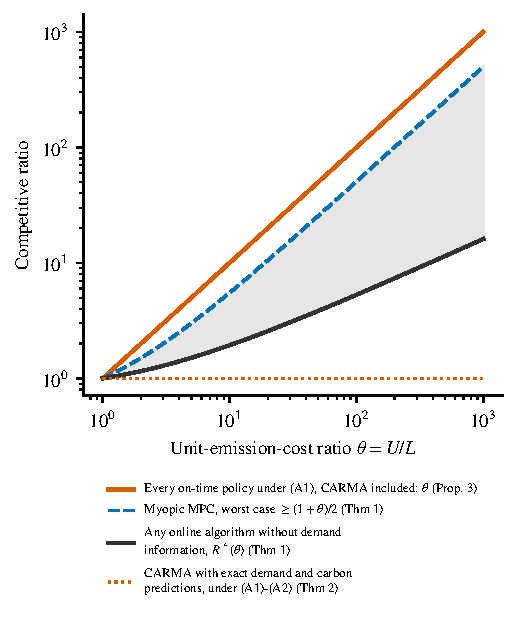
\includegraphics[width=0.62\textwidth]{fig7_ratios.pdf}
\caption{Worst-case landscape as a function of the unit-emission-cost ratio $\theta=U/L$. The curves refer to different information regimes. Without information about future demand, no online algorithm can lie below $R^*(\theta)$, even with exact carbon forecasts (Theorem~\ref{thm:lb}), and myopic MPC can be driven to $(1+\theta)/2$. Given a backstop (A1), every policy that meets its deadlines, CARMA included, is within $\theta$ (Proposition~\ref{prop:robust}). With exact predictions of \emph{both} demand and carbon and an episode within the planning window (A1--A2), CARMA is optimal (Theorem~\ref{thm:carma}).}
\label{fig:ratios}
\end{figure}

\subsection{Fair carbon attribution among sites}\label{sec:fair}

Pooling capacity reduces total emissions but redistributes them. Work submitted in London is executed in South Scotland, and Scottish jobs may be displaced by it. The organizations that operate the sites, or the business units that submit the jobs, therefore need an attribution of the pooled emissions that each of them can accept. This is an \emph{internal} allocation problem, like carbon transfer pricing between units. It is distinct from external GHG Protocol reporting, where Scope~2 emissions are reported by the entity that consumes the electricity~\cite{ghg2015scope2}.

We model the allocation as a cooperative game. The players are the sites $\mathcal S$. A coalition $C\subseteq\mathcal S$ pools the capacity of its sites and serves the jobs submitted at them. Its stand-alone value $c(C)$ is the optimum of (\ref{eq:obj})--(\ref{eq:cap}) restricted to those jobs and sites, which includes the lateness penalty if the coalition cannot serve its own jobs on time. An attribution $\phi\in\mathbb{R}^{|\mathcal S|}$ is \emph{budget-balanced} if $\sum_o\phi_o=c(\mathcal S)$. It is in the \emph{core} if $\sum_{o\in C}\phi_o\le c(C)$ for every coalition $C$. A core attribution gives no group of sites a reason to leave the pool and schedule on its own.

Let $(\lambda,\nu,\mu)$ be optimal dual variables of the grand-coalition problem: $\lambda_j$ for the work constraint (\ref{eq:work}), $\nu_{jt}\le 0$ for the width constraint (\ref{eq:width}) and $\mu_{st}\le 0$ for the capacity constraint (\ref{eq:cap}). The \emph{dual carbon attribution} is
\begin{equation}\label{eq:phi}
\phi_o=\sum_{j:\,o_j=o}\Big(\lambda_j w_j+\sum_t \nu_{jt}m_j\Big)+\sum_t\mu_{ot}K_o(t).
\end{equation}
Site $o$ is charged the carbon shadow price of the work it submits and is credited ($\mu\le 0$) with the shadow value of the capacity it contributes. A site whose clean capacity is worth more than the emissions of its own jobs therefore receives a net credit, that is, a negative internal charge.

\begin{theorem}[Core-stable carbon attribution]\label{thm:core}
The attribution (\ref{eq:phi}) is budget-balanced and in the core of the pooling game. In particular, it is individually rational: no site is charged more than its stand-alone optimum $c(\{o\})$.
\end{theorem}

The result follows from Owen's theorem on linear production games~\cite{owen1975core}; games defined by network flows are known to be totally balanced~\cite{kalai1982totally}. It concerns the penalized hindsight game defined in Section~\ref{sec:fair}. Core stability is one requirement of an acceptable allocation; it does not imply uniqueness, incentive compatibility or other notions of fairness, and it does not extend automatically to the realized emissions of an online policy. The duals are those of the hindsight problem, which suits after-the-fact accounting. They are available as the optimal node potentials of the min-cost flow; in our experiments we obtain them from an LP solver. Optimal duals need not be unique, so Section~\ref{sec:res_fair} reports the range of (\ref{eq:phi}) over all optimal duals. It also compares the dual attribution with the Shapley value~\cite{shapley1953value}, which is budget-balanced but not guaranteed to lie in the core, and with simpler rules. The simpler rules are \emph{origin-based} (each site is charged the emissions of its own jobs wherever they ran), \emph{host-based} (each site is charged the emissions of the work it executes, the analog of location-based Scope~2 reporting), and proportional rules.

\section{Results}\label{sec:results}

\FloatBarrier
\subsection{Carbon-intensity data and forecasts}\label{sec:res_forecast}

Fig.~\ref{fig:data} shows the regional intensities. Over 2022--2024, mean intensity was 37~gCO$_2$/kWh in South Scotland, 58 in North West England, 156 in the West Midlands and 163 in London. The regional means indicate large spatial heterogeneity, and it persists hour by hour: the spread between the cleanest and the dirtiest of the four sites has a median of 156~gCO$_2$/kWh and exceeds 54~g in 90\% of hours. This is what makes spatial shifting attractive. Annual mean intensities declined at every site; London's fell from 202~gCO$_2$/kWh in 2022 to 125 in 2024. Diurnal profiles peak in the early evening (around 18:00 UTC), and the profile of South Scotland is much flatter than those of the southern sites. The four series are positively correlated (pairwise correlations between 0.51 and 0.87), because national wind output drives all of them.

\begin{figure}[!htbp]
\centering
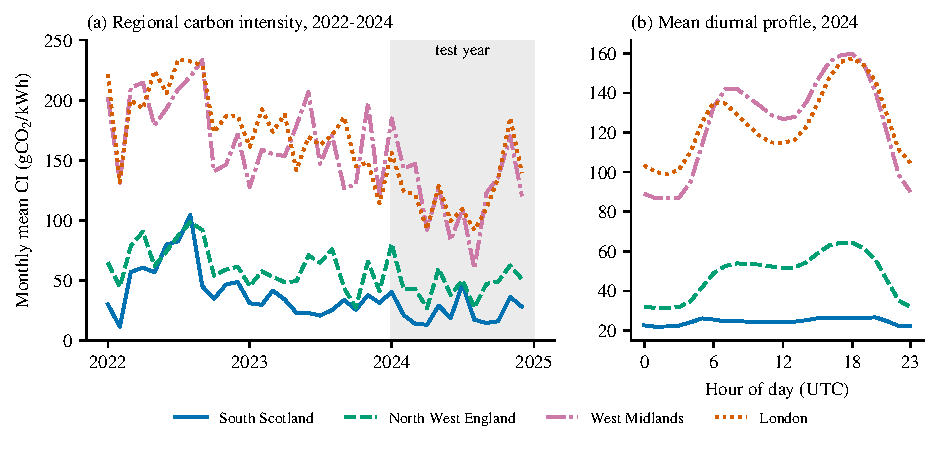
\includegraphics[width=\textwidth]{fig2_data.pdf}
\caption{Hourly carbon intensity of the four candidate sites (NESO regional data). (a) Monthly means, 2022--2024; the shaded area is the out-of-sample test year. (b) Mean diurnal profile in 2024 (UTC).}
\label{fig:data}
\end{figure}

The forecaster was trained on 1.24 million (issue time, site, horizon) samples in about one minute. In 2024 its mean absolute error (MAE), averaged over horizons and sites, is 31.7~gCO$_2$/kWh, against 35.3 for persistence and 40.9 for a seasonal-naive forecast. The advantage is 23--25\% at horizons of 1--6 hours, and the difference is significant at all English sites up to 18 hours in Diebold--Mariano tests~\cite{diebold1995comparing}. Day-ahead skill is limited, because no weather inputs are used. Adaptive recalibration keeps the annual coverage of the upper bounds within 0.003 of target despite the 2024 decarbonization drift. \appref{app:forecast} gives the full evaluation (accuracy by horizon and site, coverage, pinball loss).

\FloatBarrier
\subsection{Hyperparameter tuning}\label{sec:tuning}

All policies were tuned on 13 validation weeks (October--December 2023, $\rho\in\{0.3,0.5,0.7\}$), separately for each regime. Fig.~\ref{fig:tuning} shows the spatio-temporal regime. Anticipating demand helps across the whole grid: every tested configuration beats myopic MPC, whose mean gap to the oracle is 22.3\%. The gap is smallest around $\kappa=1$, where expected demand is anticipated without inflation: 9.3\% for $\ell=12$ and 9.1\% for $\ell=18$. Over-anticipation ($\kappa=1.25$ with $\ell=18$) reserves too much clean capacity and is penalized (12.4\%). We selected $\kappa=1$ and $\ell=12$ hours, resolving configurations within 0.25 percentage points of the best toward the shorter look-ahead. In the temporal-only regime, anticipation brings no benefit. The best configuration ($\kappa=0.5$, $\ell=6$; 4.29\%) is indistinguishable from MPC (4.29\%), and larger $\kappa$ is slightly worse. For MPC-Protect, the best protection level was $r=0.3$ with $\tau=1$~h in the spatio-temporal regime (21.3\% against 22.3\% for MPC). In the temporal-only regime every protection level was worse than MPC (at best 5.9\%). For Scenario-MPC, $K=8$ scenarios with $\ell=12$ gave 9.0\%, against 9.3\% with $K=4$ and 12.5--12.7\% with $\ell=6$.

\begin{figure}[!htbp]
\centering
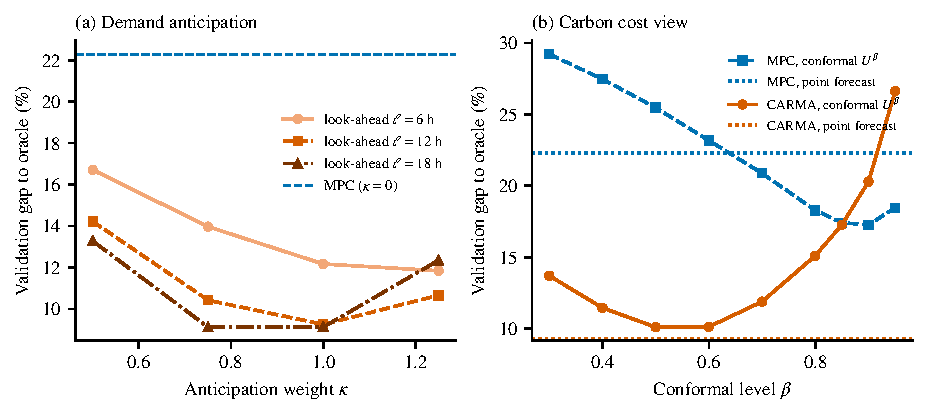
\includegraphics[width=\textwidth]{fig6_tuning.pdf}
\caption{Validation results for the spatio-temporal regime (2023-Q4, mean over 13 weeks and three load levels). (a) Gap to the oracle as a function of the anticipation weight $\kappa$ and look-ahead $\ell$, using point forecasts. (b) Effect of the carbon cost view: conformal quantiles $U^\beta$ against point forecasts, for myopic MPC and for CARMA ($\kappa=1$, $\ell=12$).}
\label{fig:tuning}
\end{figure}

The cost view interacts with anticipation (Fig.~\ref{fig:tuning}b). For myopic MPC, high conformal levels help. The gap falls from 25.5\% at $\beta=0.5$ to 17.3\% at $\beta=0.9$ and rises again at $\beta=0.95$ (18.5\%), against 22.3\% with point forecasts. For CARMA, every conformal level is worse than the point forecast: the best, $\beta=0.5$, gives 10.1\% against 9.3\%. The mechanism is not a uniform risk premium. On the validation weeks, the $\beta=0.6$ view lies on average between 1.5~g below and 3.9~g above the point forecast at South Scotland, North West England and London, but 14.5~g above it at the volatile West Midlands site. The offset also grows with the horizon, and at $\beta=0.8$ it reaches 23--95~g at a 24-hour horizon. High levels therefore make distant hours and volatile sites look dirtier, so the planner runs work now and at stable sites, which keeps future clean capacity free. For a myopic planner this is a crude form of anticipation. Once CARMA represents future demand explicitly, the same distortion double-counts it and gives up useful deferrals. The selected CARMA therefore uses point forecasts. For the test we keep MPC+conformal at $\beta=0.9$ and CARMA+conformal at $\beta=0.5$ (spatio-temporal) as ablations. In the temporal-only regime, the best conformal views were $\beta=0.6$ for MPC and $\beta=0.5$ for CARMA.

\FloatBarrier
\subsection{Out-of-sample scheduling performance}\label{sec:res_main}

Tables~\ref{tab:main} and~\ref{tab:main_t} report results for the 52 test weeks of 2024, with three independent workload traces per week. Weekly traces contain on average 917, 1{,}527 and 2{,}141 jobs (69{,}400, 115{,}400 and 162{,}000 server-hours) at $\rho=0.3$, 0.5 and 0.7. Fig.~\ref{fig:gap} shows the gaps to the oracle.

\begin{table}[p]
\centering
\caption{Out-of-sample results in the spatio-temporal regime (migration allowed), 52 weeks of 2024 $\times$ 3 traces. Emis.: mean weekly operational emissions (tCO$_2$, attributional). Red.: reduction relative to ASAP-Local (\%). Gap: excess over the clairvoyant oracle (\%). Adj.: service-adjusted gap, in which late work is additionally charged at the episode's largest local unit cost and the oracle minimizes the same objective. Late: share of work outstanding at its deadline (\%). Mig.: share of work executed away from its origin (\%). ms: mean decision time per hour (one CPU core). $p$: two-sided moving-block bootstrap test of the mean paired weekly difference in gap against CARMA, Holm-adjusted jointly over all comparisons in Tables~\ref{tab:main} and~\ref{tab:main_t}. Red.\ and Gap are means of per-episode ratios. The best gap among implementable online policies is in bold.}
\label{tab:main}
\footnotesize\setlength{\tabcolsep}{3.5pt}
\begin{tabular}{llrrrrrrrl}
\toprule
Load & Policy & Emis. & Red. & Gap & Adj. & Late & Mig. & ms & $p$ \\
\midrule
\inputtable{table_main_st.tex}
\bottomrule
\end{tabular}
\end{table}

\begin{table}[p]
\centering
\caption{Out-of-sample results in the temporal-only regime (no migration), 52 weeks of 2024 $\times$ 3 traces. Columns as in Table~\ref{tab:main}. Greedy-Spatial is omitted because without migration it coincides with ASAP-Local.}
\label{tab:main_t}
\footnotesize\setlength{\tabcolsep}{3.5pt}
\begin{tabular}{llrrrrrrl}
\toprule
Load & Policy & Emis. & Red. & Gap & Adj. & Late & ms & $p$ \\
\midrule
\inputtable{table_main_t.tex}
\bottomrule
\end{tabular}
\end{table}

\begin{figure}[!htbp]
\centering
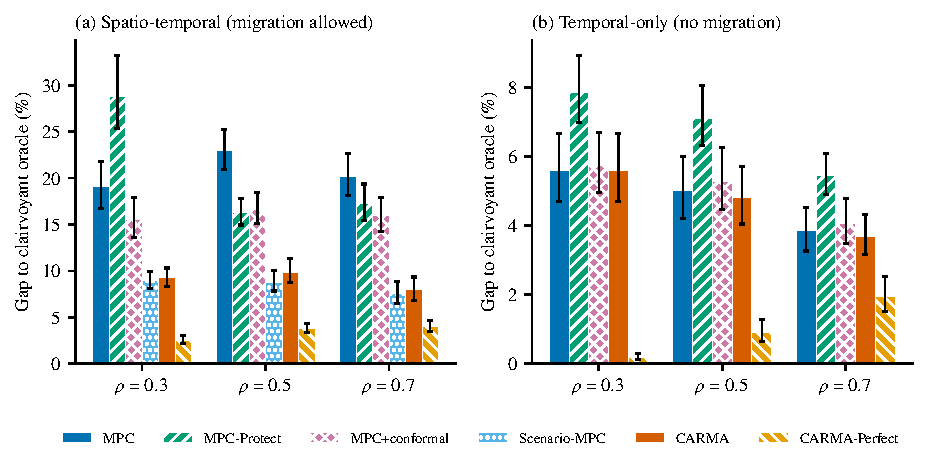
\includegraphics[width=\textwidth]{fig4_gap.pdf}
\caption{Gap to the clairvoyant oracle. Mean over the 52 test weeks of 2024 (week means of three traces) with 95\% moving-block bootstrap intervals, for MPC, MPC-Protect, MPC+conformal, Scenario-MPC (run in the spatio-temporal regime only), CARMA and CARMA-Perfect. ASAP-Local (gap 73--284\% with migration, 10--22\% without), Greedy-Spatial, Forecast-Reserve and MPC-Perfect are omitted for legibility and listed in Tables~\ref{tab:main} and~\ref{tab:main_t}. Bar patterns repeat the legend colors.}
\label{fig:gap}
\end{figure}

\paragraph{Spatio-temporal regime} With migration allowed, the oracle cuts attributional emissions relative to ASAP-Local by 71.8\%, 58.2\% and 41.1\% at $\rho=0.3$, 0.5 and 0.7. Greedy-Spatial realizes only part of this potential (gaps of 38--67\%), because it has no temporal flexibility and floods the cleanest site with whatever arrives first. The forecast-driven planners without demand information come closer. Forecast-Reserve has gaps of 24--27\% and MPC 19--23\%. MPC+conformal (15.5--16.6\%) is the best of them at $\rho=0.3$ and 0.7 and MPC-Protect at $\rho=0.5$ (16.3\%); at $\rho=0.3$, where clean capacity is rarely scarce, the protection level wastes it and MPC-Protect is worse than MPC (28.8\%). CARMA reduces emissions by 69.3\%, 54.3\% and 36.6\% and has gaps of 9.3\%, 9.8\% and 8.0\%. Relative to MPC this is a further emission reduction of 7.7\%, 9.7\% and 9.1\%. Its advantage over the best of these baselines at each load is 6.3 (95\% block-bootstrap CI 4.5--8.2), 6.5 (5.2--7.4) and 8.0 (6.9--9.0) percentage points of gap, and CARMA emits less than MPC in 51, 51 and 52 of the 52 week-means. Scenario-MPC, which uses the same demand information in a two-stage stochastic program, does slightly better than CARMA: its gaps are 9.0\%, 8.8\% and 7.5\%, lower by 0.3 (0.2--0.5), 1.0 (0.9--1.3) and 0.4 (0.3--0.6) points, and CARMA is better in only 19, 5 and 8 weeks. Scenario-MPC, however, needs 250--1{,}450~ms per decision against 21--40~ms for CARMA, 12--37 times longer, and solves a general LP instead of a network flow. CARMA thus captures most of the value of demand information, 10--13 points of gap against MPC, and gives up 0.3--1.0 points against a stochastic program with the same information. Block lengths of two and eight weeks give the same conclusions.

CARMA also finishes more work on time under heavy load. At $\rho=0.7$, 0.02\% of its work is late (Scenario-MPC 0.02\%), against 1.9\% for MPC, 0.7\% for MPC-Protect, 1.1\% for Forecast-Reserve and 4.5\% for ASAP-Local. The service-adjusted gap therefore widens the difference: 8.0\% for CARMA against 18.1--31.2\% for the forecast-driven baselines without demand information. CARMA migrates about the same share of work as MPC (32--70\%), whereas MPC-Protect migrates more (38--81\%). CARMA's advantage thus comes from better timing of the use of scarce clean capacity, not from moving more data. For the fleet of 1{,}700 batch servers at $\rho=0.5$, CARMA emits 0.31~tCO$_2$ per week less than MPC, about 16~tCO$_2$ per year, and 3.22~tCO$_2$ per week less than carbon-agnostic operation. These absolute figures scale with fleet size. Two test weeks contain gap-filled hours (Section~\ref{sec:data}); excluding them changes CARMA's gaps by at most 0.2 points and no ranking.

\begin{figure}[!htbp]
\centering
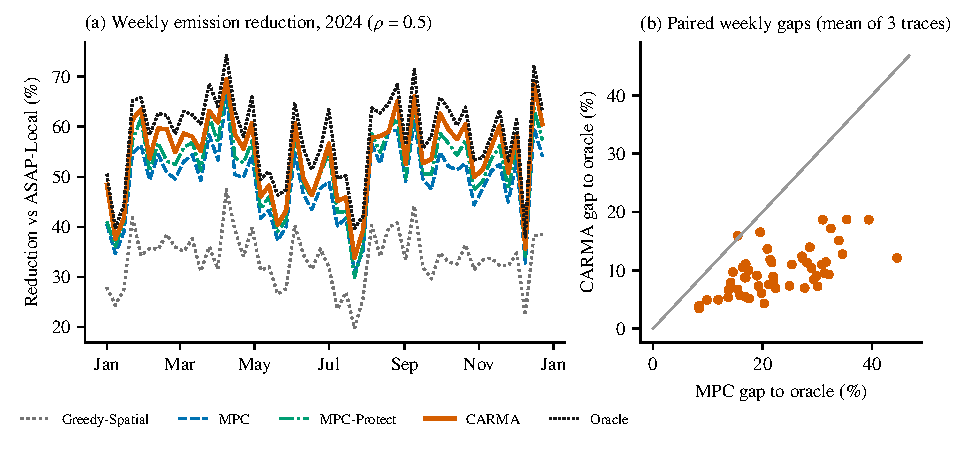
\includegraphics[width=\textwidth]{fig5_weekly.pdf}
\caption{Weekly results in 2024 (spatio-temporal regime, $\rho=0.5$, means of three traces). (a) Emission reduction relative to ASAP-Local. (b) Paired weekly gaps to the oracle; points below the diagonal are weeks in which CARMA outperforms MPC.}
\label{fig:weekly}
\end{figure}

\paragraph{Value of information} The clairvoyant variants separate two sources of loss. With perfect intensity forecasts, the myopic MPC-Perfect still has gaps of 16.7\%, 21.3\% and 18.8\%. Perfect carbon foresight is thus worth only 1.4--2.4 percentage points to a myopic planner, whereas anticipating demand is worth 9.8--13.2 points (MPC versus CARMA). With both, CARMA-Perfect comes within 2.5--4.0\% of the oracle. CARMA-Perfect has exact carbon forecasts but still uses the average demand profile, so it is not the exact-prediction case of Theorem~\ref{thm:carma}. The two kinds of information are complementary. Once demand is anticipated, forecast accuracy is worth 4.0--6.8 points (CARMA versus CARMA-Perfect), about three to four times more than for the myopic planner. The ranking is stable across seasons (Fig.~\ref{fig:weekly}a), although the level of achievable reductions varies from week to week with wind conditions.

\paragraph{Temporal-only regime} Without migration (Table~\ref{tab:main_t}), each job can only move in time at its origin. Achievable reductions are much smaller: the oracle saves 18.0\%, 15.1\% and 8.7\%. MPC and CARMA are within 3.7--5.6\% of the oracle. They are statistically indistinguishable at $\rho=0.3$ (difference 0.01 points, CI $-0.01$ to 0.02). CARMA is slightly better at higher loads, by 0.20 (0.13--0.30) and 0.15 (0.07--0.25) points. Both are better than Forecast-Reserve and MPC-Protect. Anticipation brings little benefit here, because each site's capacity serves only its own jobs, and flexible and urgent work rarely compete for the same clean hours in a way that deferral cannot absorb. The remaining loss is due almost entirely to forecast error: the Perfect variants close the gap to 0.2--2.3\%. Heavy load exposes a trade-off that the emission metric hides. At $\rho=0.7$, the capacity at the origin sites is itself insufficient, and every carbon-aware policy delays work: 9.3\% of CARMA's work and 11.8\% of MPC's is late, against 4.5\% for ASAP-Local. In this cell the emission gap is not an optimality gap, because the oracle meets deadlines. Under the service-adjusted metric, carbon-agnostic operation (22.5\%) is preferable to MPC (42.1\%) and CARMA (32.9\%). Without migration and near saturation, temporal shifting should therefore be restricted or combined with explicit service constraints.

\paragraph{Computation} A CARMA decision takes 7--40~ms on one CPU core, against 1--7~ms for MPC; the difference comes from the ghost jobs, which enlarge the planning network. Scenario-MPC needs 0.25--1.5~s. Both are fast enough for hourly decisions in this fleet, but the cost of the stochastic program grows with the number of scenarios and jobs, while CARMA remains a single network flow. A clairvoyant weekly oracle with up to about 2{,}800 jobs is solved in under one second by the flow solver.

\FloatBarrier
\subsection{Trace-derived workload}\label{sec:res_trace}

Table~\ref{tab:trace} reports the experiment with the trace-derived workload. Arrivals and job sizes come from the Alibaba trace, and the demand information of CARMA and Scenario-MPC comes from different days, so the profile underestimates demand by 28\% and cannot anticipate bursts. The evaluation covers the four trace days paired with 52 carbon windows of 2024, with three draws of origins and deadlines each, and 3{,}072 evaluated job batches (65{,}300 server-hours) per window. Real, bursty demand makes all policies worse than in the synthetic experiment, but the ranking is unchanged. CARMA has a gap of 21.2\%, against 27.5\% for MPC-Protect, the best baseline without demand information, and 36.8\% for MPC. Carbon foresight again matters less than demand anticipation: MPC-Perfect reaches only 34.1\%. CARMA's advantage over MPC-Protect is 6.3 percentage points (95\% CI 4.6--8.3; CARMA better in 42 of 52 carbon windows, $p<0.001$). Scenario-MPC is again slightly better than CARMA, by 1.4 points (0.6--1.8; gap 19.7\%), at 1.2~s per decision against 48~ms. The bias of the learned profile costs 3.0 points (CI 1.1--4.0): CARMA with a profile estimated in-sample from the evaluation days reaches 18.2\%. With the biased profile but perfect carbon forecasts, the gap would fall by 3.8 points (CARMA-Perfect, 17.4\%). The remaining distance to the oracle reflects bursts that no profile anticipates. CARMA also keeps late work low (0.09\%, against 0.66\% for MPC).

Batching pools the widths of jobs with different work-to-width ratios and therefore relaxes the problem. With finer batches that also separate jobs by run-length class (about twice as many batches, one draw per carbon window), the oracle emits 2.5\% more, so batching makes the benchmark slightly optimistic. The ranking is unchanged: gaps are 20.0\% for CARMA, 26.2\% for MPC-Protect and 34.3\% for MPC, and CARMA's advantage over MPC-Protect is 6.3 points (4.8--7.8). The 156 episodes share one demand chronology, so the trace result is evidence about robustness to carbon conditions and to a biased profile for this workload, not a sample of independent demand weeks.

\begin{table}[!htbp]
\centering
\caption{Trace-derived workload (Alibaba 2018 cluster trace, days 5--8; demand information from days 1--4), paired with 52 carbon windows of 2024 $\times$ 3 draws of origins and deadlines; spatio-temporal regime, $\rho=0.5$. Emissions are per four-day window. Columns as in Table~\ref{tab:main}; the service-adjusted gap is omitted; $p$ values are Holm-adjusted within this table.}
\label{tab:trace}
\footnotesize\setlength{\tabcolsep}{3.5pt}
\begin{tabular}{lrrrrrrl}
\toprule
Policy & Emis. & Red. & Gap & Late & Mig. & ms & $p$ \\
\midrule
\inputtable{table_trace.tex}
\bottomrule
\end{tabular}
\end{table}

\FloatBarrier
\subsection{Sensitivity analysis}\label{sec:sens}

Table~\ref{tab:sens} varies one factor at a time around the base case: spatio-temporal regime, $\rho=0.5$, $\upsilon=0.3$, $\eta=0.02$~kWh/GB, capacities 300/400/400/600. Each setting uses 26 alternating test weeks of 2024 with two fresh workload traces per week. All policies keep their base-case hyperparameters.

\begin{sidewaystable}
\centering
\caption{Sensitivity analysis (spatio-temporal regime; 26 alternating weeks of 2024 $\times$ 2 traces per setting). Oracle red.: emission reduction of the oracle relative to ASAP-Local (\%). Gap columns: excess over the oracle (\%). Wins: weeks in which CARMA emits less than MPC. Late: share of late work (\%), MPC / CARMA. $^{a}$Busy servers draw 0.2~kWh above an idle draw of 0.2~kWh per server-hour that every batch server incurs regardless of the schedule. $^{b}$Schedules are made with average intensities, but emissions are accounted with the stylized marginal emission factor of Section~\ref{sec:sens}, and the oracle optimizes marginal emissions.}
\label{tab:sens}
\footnotesize\setlength{\tabcolsep}{3pt}
\begin{tabular}{lrrrrrrrr}
\toprule
 & Oracle & \multicolumn{5}{c}{Gap to oracle (\%)} & Wins vs & Late (\%) \\
\cmidrule(lr){3-7}
Setting & red. & Greedy & Reserve & MPC & Protect & CARMA & MPC & MPC/CARMA \\
\midrule
\inputtable{table_sens.tex}
\bottomrule
\end{tabular}
\end{sidewaystable}

\paragraph{Workload and network} CARMA has the smallest gap of the online policies compared here in every setting (Scenario-MPC is omitted from the sensitivity analysis because of its computational cost). Except under marginal accounting (see the paragraph on marginal emissions of this section), it emits less than MPC in all 26 weeks of each setting. The benefit of anticipation grows with the share of urgent work, because urgent arrivals are precisely the demand that myopic planners crowd out. With $\upsilon=0.5$, CARMA's gap is 6.7\% against 15.3\% for MPC-Protect and 21.5\% for MPC. With $\upsilon=0.1$, it is 12.0\% against 16.4\% and 23.3\%. The ranking is unchanged over a twelve-fold range of transmission energy intensity ($\eta=0.005$--$0.06$~kWh/GB), and the migrated share of CARMA's work stays at 49--51\%.

\paragraph{Capacity layout} Arrival rates are rescaled with the fleet's capacity, so the offered load stays at $\rho=0.5$ of the new capacity. The advantage does not depend on the chosen layout. When the clean South Scotland site is halved (150 servers) or doubled (600), or London's capacity is doubled, CARMA's gap stays at 9.3--9.5\%. The gaps of MPC (22--29\%) and MPC-Protect (16.9--18.9\%) stay about two to three times larger. More clean capacity raises the oracle's reduction (from 52.4\% to 69.2\%), but a myopic planner still misallocates it.

\paragraph{Misspecified demand profile} CARMA's ghost jobs come from a profile learned at $\rho=0.5$. When the actual load is 20\% higher ($\rho=0.6$), so that CARMA under-anticipates, its gap is 8.6\% against 19.0\% for MPC-Protect and 24.1\% for MPC. When the actual load is 20\% lower ($\rho=0.4$), CARMA over-anticipates and reserves more clean capacity than needed. Its gap rises to 12.2\%, but it still beats MPC-Protect by 3.7 points (15.9\%) and MPC by 11.2 points. The trace experiment of Section~\ref{sec:res_trace} adds a real profile that underestimates demand by 28\%. Because ghost work carries a lower penalty than real work, the planner never plans real work late in order to serve ghost demand. Without a backstop, however, a misprediction can still delay real work once capacity is exhausted (Section~\ref{sec:guarantees}); the late-work column of Table~\ref{tab:sens} tracks this.

\paragraph{Always-on servers} If every batch server draws idle power whether or not it is busy, a large part of the emissions no longer depends on the schedule. The achievable reduction falls to 18.5\% for the oracle and 17.3\% for CARMA. The ranking is unchanged (gaps of 1.5\% for CARMA, 2.6\% for MPC-Protect and 3.6\% for MPC). Carbon-aware scheduling is therefore most valuable when it is combined with right-sizing, so that deferred work actually reduces the number of powered servers~\cite{lin2013dynamic}.

\paragraph{Marginal emissions} All sites are in one GB market, where gas-fired plant is usually the marginal generator~\cite{staffell2017measuring,hawkes2010estimating}. Moving load between regions then mainly changes \emph{which} region is assigned the average mix, and it abates emissions physically only when low-carbon output would otherwise be curtailed. We therefore account emissions with a stylized marginal emission factor (MEF). The MEF is 394~gCO$_2$/kWh (combined-cycle gas) in every hour except two cases where it is zero. For South Scotland it is zero when Scotland is nearly carbon-free (below 25~g) while GB-wide intensity exceeds 100~g, a proxy for export-constrained hours; this holds in 27\% of hours. For all sites it is zero when GB-wide intensity is below 50~g (4\% of hours). Under this accounting the picture changes substantially. The oracle cuts marginal emissions by only 13.8\%, and CARMA by 7.5\%. The forecast-driven policies are within 7.9--10.7\% of the marginal oracle. CARMA is still the best of them, but its advantage over MPC shrinks to 0.6 points (block-bootstrap CI 0.1--0.9; $p=0.003$ after Holm correction; CARMA better in 18 of 26 weeks). The schedules were optimized for average intensity, not for the MEF, and the MEF itself is a proxy with fixed thresholds that has not been validated against dispatch or curtailment data. Under this proxy, most of the attributional reductions reported in Sections~\ref{sec:res_main}--\ref{sec:res_trace} would be reallocations within the GB system. The physical benefit depends on whether shifting absorbs otherwise-curtailed low-carbon output or changes the marginal generator between hours, and a scheduler should be driven by a validated marginal signal when that is the goal.

\FloatBarrier
\subsection{Other grids and continents}\label{sec:multigrid}

To test whether the findings depend on the British grid, we repeat the experiment on the four further fleets of Table~\ref{tab:fleets}: Europe, the United States, Brazil and a fleet with one site on each of four continents. The last fleet spans time zones from UTC$-8$ to UTC$+12$, so jobs submitted during one region's working day can run in another region's night. For every fleet we retrain the forecaster and tune CARMA, MPC-Protect and the conformal view of MPC on the fleet's own validation weeks (Section~\ref{sec:data}), so no method keeps a setting tuned on Great Britain. Table~\ref{tab:multigrid} and Fig.~\ref{fig:multigrid} summarize the results at $\rho=0.5$, and \appref{app:multigrid} gives all loads.

\begin{table}[!htbp]
\centering
\caption{Results on five grids ($\rho=0.5$, migration allowed; 52 test weeks of 2024). Red.: emission reduction of the oracle relative to ASAP-Local (\%). Columns 3--6: gap to the oracle (\%). Best-base.: gap of the best of Greedy-Spatial, Forecast-Reserve, MPC, MPC-Protect and MPC+conformal minus CARMA's gap (points). Wins: weeks in which CARMA emits less than MPC. Scenario-MPC gap / CARMA gap on the 26 alternating weeks on which Scenario-MPC was run (one trace). Great Britain: main experiment (three traces per week); other fleets: two traces per week.}
\label{tab:multigrid}
\scriptsize\setlength{\tabcolsep}{2.5pt}
\begin{tabular}{lrrrrrrrrr}
\toprule
Fleet & \makecell{Oracle\\red.} & MPC & \makecell{MPC-\\Prot.} & \makecell{MPC+\\conf.} & CARMA & \makecell{Scen.-MPC /\\CARMA} & \makecell{Best-\\base.} & Wins & \makecell{CARMA-\\Perfect} \\
\midrule
\inputtable{table_multigrid.tex}
\bottomrule
\end{tabular}
\end{table}

\begin{figure}[!htbp]
\centering
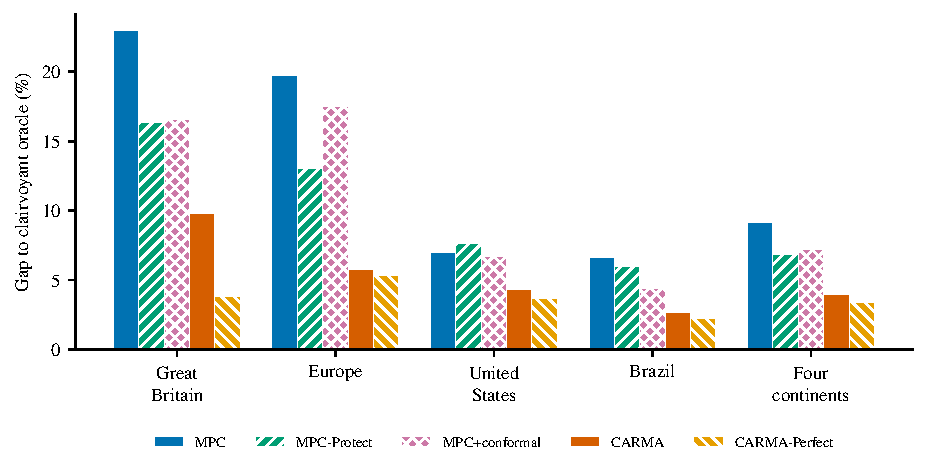
\includegraphics[width=\textwidth]{fig10_multigrid.pdf}
\caption{Gap to the clairvoyant oracle on five grids ($\rho=0.5$, migration allowed, 52 test weeks; Great Britain with three traces per week, the other fleets with two). Scenario-MPC, which was run on a subset of weeks, is shown in Table~\ref{tab:multigrid}. Bar patterns repeat the legend colors.}
\label{fig:multigrid}
\end{figure}

CARMA has the smallest gap of all implementable policies without a stochastic program on every grid and at every load. At $\rho=0.5$ its gaps are 5.8\% in Europe, 4.3\% in the United States, 2.7\% in Brazil and 4.0\% for the four-continent fleet, against 13.0\%, 6.7\%, 4.4\% and 6.8\% for the best baseline without demand information. CARMA's advantage is 7.3 (95\% block-bootstrap CI 6.2--8.7), 2.4 (2.0--2.9), 1.7 (1.2--2.3) and 2.8 (2.4--3.3) points, and it emits less than MPC in all 52 weeks on each grid. Which baseline is best varies. MPC-Protect is the best baseline in Europe and for the four-continent fleet and MPC+conformal in the United States and Brazil, whereas at $\rho=0.3$ MPC-Protect is worse than plain MPC on all four grids. Over all 15 fleet-load cells the advantage over the best baseline ranges from 1.3 to 7.3 points. It is smaller than in Great Britain (6.3--8.0 points) in the United States and Brazil, and the gap of myopic MPC is correspondingly smaller (7.0\% and 6.6\% at $\rho=0.5$, against 23.0\% in Great Britain). A possible reason is that the sites of these two fleets are closer to each other relative to their mean intensity: the median relative spread between the cleanest and the dirtiest site, $(\max-\min)/\text{mean}$ in 2024, is 1.25 in the United States and 1.27 in Brazil, against 1.71 in Great Britain, 1.80 for the four-continent fleet and 2.06 in Europe, where the nuclear-based French and the coal-based Polish grids are far apart. The advantage broadly follows this spread, but five grids cannot establish a relation. Perfect carbon forecasts would reduce CARMA's gap by a further 0.4--0.6 points at $\rho=0.5$, so the remaining distance to the oracle is mostly due to demand uncertainty. CARMA's late work stays below 0.03\% of work at every load.

The emission reductions follow the same pattern. At $\rho=0.5$ CARMA reduces emissions relative to carbon-agnostic operation by 60.9\% in Europe, 31.8\% in the United States, 35.9\% in Brazil and 54.2\% for the four-continent fleet, compared with 63.0\%, 34.6\%, 37.5\% and 56.0\% for the oracle. These are attributional reductions under production-based intensities and inherit the caveats of the marginal analysis above.

\paragraph{Scenario-MPC} The stochastic lookahead is level with CARMA on three of the new grids. Its gap is 0.09 points above CARMA's in Europe (CI $-0.24$ to 0.42), 0.15 points above it in Brazil (0.01--0.34) and 0.20 points above it for the four-continent fleet ($-0.05$ to 0.55). It is better by 0.44 points in the United States (0.25--0.69), and by 1.0 points in Great Britain on the same subset of weeks. It needs 0.9~s per decision against 33~ms for CARMA, 26--27 times longer. The overall picture from the British experiment therefore holds on other grids: CARMA captures nearly all of the value of demand information at a small fraction of the computing cost of a scenario-based program.

\paragraph{Reversed capacity layout} In all fleets the cleanest site has the least capacity and the smallest share of job origins, as in Great Britain. To check that the result does not depend on this layout, we reverse both assignments, so that the cleanest site is the largest. CARMA's gap is then 6.7\%, 6.0\%, 2.6\% and 3.6\% in Europe, the United States, Brazil and the four-continent fleet, against 18.9\%, 12.4\%, 4.6\% and 6.6\% for the best baseline without demand information (26 alternating weeks, $\rho=0.5$; advantages of 12.1, 6.4, 2.0 and 3.0 points). The oracle's reductions are 61.7\%, 40.7\%, 28.7\% and 46.3\% in this layout, and CARMA's 59.2\%, 37.2\%, 26.9\% and 44.4\%. The ranking of the policies is unchanged.

\paragraph{Forecasts} The forecaster is more accurate than persistence on every grid (mean absolute error of 30.1 against 52.4~gCO$_2$/kWh in Europe, 19.8 against 34.8 in the United States, 7.3 against 12.3 in Brazil and 10.6 against 21.7 for the four-continent fleet), and the adaptively recalibrated upper bounds cover within 0.012 of the target at every level.


\FloatBarrier
\subsection{Robustness to prediction errors}\label{sec:res_robust}

We test how CARMA degrades as its predictions deteriorate on every fourth test week of 2024 (13 weeks, $\rho=0.5$, migration allowed, fresh workload traces). Controlled errors are injected into the two kinds of prediction (Fig.~\ref{fig:robust}). These experiments do not satisfy the assumptions of the bound in Theorem~\ref{thm:carma}, so they probe the degradation profile empirically.

\begin{figure}[!htbp]
\centering
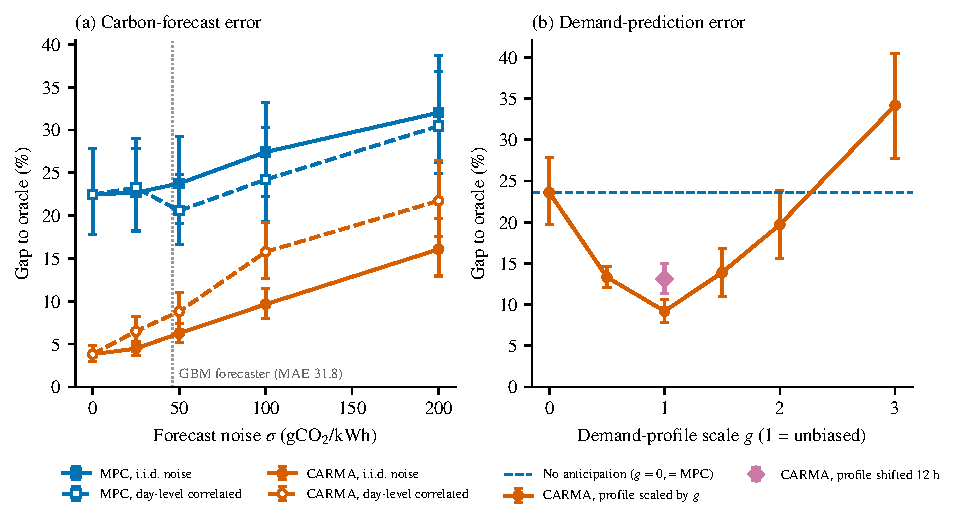
\includegraphics[width=\textwidth]{fig8_robust.pdf}
\caption{Degradation under controlled prediction errors (13 test weeks of 2024, $\rho=0.5$, migration allowed; means with 95\% confidence intervals). (a) Carbon-intensity forecasts replaced by the realized values plus Gaussian noise of standard deviation $\sigma$. The noise is either independent across issue times and horizons (solid) or shared by all forecasts of the same site and target day (dashed, open markers). (b) Demand profile scaled by $g$, or shifted by 12 hours so that arrivals are predicted at the wrong time of day.}
\label{fig:robust}
\end{figure}

\paragraph{Carbon-forecast error} With exact forecasts, CARMA's gap is 3.8\% and MPC's 22.5\%. Independent noise is comparatively benign: CARMA's gap rises smoothly to 4.5\%, 6.3\%, 9.7\% and 16.1\% at $\sigma=25$, 50, 100 and 200~gCO$_2$/kWh. Noise that persists over a whole target day, as when a weather front is missed, is more damaging. The gaps are then 6.5\%, 8.8\%, 15.8\% and 21.7\%, because the planner cannot average out the error by re-planning. MPC deteriorates from 22.5\% to 30.5--32.0\% at the largest noise level. At every noise level and type, CARMA remains better than MPC with the same forecasts. Only with the most persistent large errors ($\sigma=200$) does it approach the level of MPC with \emph{perfect} forecasts. Fig.~\ref{fig:robust}a places the GBM forecaster at the noise level with the same realized MAE (31.8~gCO$_2$/kWh, $\sigma\approx46$). With the GBM forecasts, CARMA's gap on the same weeks is 9.9\%, larger than with either noise model at that error size (about 6\% and 8.5\%). The forecaster's errors, which are both serially and cross-sectionally correlated and concentrated in volatile hours, are therefore more damaging than either stylized noise model, and the degradation should not be read as merely i.i.d.

\paragraph{Demand-prediction error} Scaling the learned demand profile by $g$ produces a V-shaped response with its minimum at the unbiased profile ($g=1$, gap 9.2\%). Under-prediction by half ($g=0.5$) and over-prediction by half ($g=1.5$) cost 4.1 and 4.7 percentage points. Predicting arrivals at the wrong time of day (a 12-hour shift) costs 3.9 points. Removing anticipation ($g=0$) returns the MPC level (23.6\%). Gross over-prediction ($g=3$, three times the true demand) is worse than no anticipation (34.2\%), because CARMA then holds clean capacity for work that never arrives. A 12-hour shift keeps most of the benefit, which indicates that much of the value comes from anticipating the \emph{volume} of demand rather than its exact timing. Late work was negligible in all 325 runs (at most 0.01\% of work). The largest ratio of CARMA's emissions to the oracle's over all runs was 1.58.

\FloatBarrier
\subsection{Fair carbon attribution}\label{sec:res_fair}

We evaluate Theorem~\ref{thm:core} on the 52 test weeks at $\rho=0.5$, with the four sites as players. For every week and each of the 15 coalitions we compute the hindsight value $c(C)$, and we also run CARMA with only the coalition's sites and jobs. Each game is one 216-hour arrival episode per week: the evaluated week plus 24 hours of arrivals before and after it. Pooling pays: the hindsight optimum of the grand coalition has a penalized cost of 3.32~tCO$_2$ per episode, against 6.69 for the four sites operating separately; the emissions alone are 3.32 and 6.58~tCO$_2$. With CARMA the figures are 3.58 and 6.87. The question is how to share the reduction.

We compare six attributions. The \emph{origin-based} rule charges each site the emissions of its own jobs wherever they run. The \emph{host-based} rule, the analog of location-based Scope~2 accounting, charges each site the emissions of the work it hosts. The \emph{work-proportional} rule splits the total in proportion to submitted work, and the \emph{stand-alone proportional} rule in proportion to stand-alone emissions. The \emph{Shapley value}~\cite{shapley1953value} averages marginal contributions over all orders of joining. The \emph{dual} rule is Eq.~(\ref{eq:phi}). Because $c(C)$ includes the lateness penalty whenever a coalition cannot serve all of its work, we also evaluate an emissions-only game, in which $c(C)$ is the emissions of the hindsight schedule. Stand-alone coalitions leave work unserved in 8 of the 52 episodes (15\%), up to 256 server-hours in one episode. In that game the dual attribution is rescaled to the emissions total and is no longer covered by the theorem. For CARMA's realized emissions, the dual attribution is applied to the hindsight value and the online excess over the hindsight optimum is split in proportion to work. A check is violated when a coalition is charged more than it would emit on its own.

\begin{table}[!htbp]
\centering
\caption{Coalitional stability of carbon attributions (52 test weeks of 2024, $\rho=0.5$; one 216-hour arrival episode per week). Checks: share of the $52\times14$ (episode, proper coalition) pairs in which the coalition is charged more than its stand-alone value. Weeks: share of episodes with at least one violation. IR: share of (episode, site) pairs in which a site is charged more than its stand-alone value. Neg.: share of (episode, site) pairs with a net credit. Max.\ exc.: largest violation (tCO$_2$). Panel (a) uses the penalized values $c(C)$ of Theorem~\ref{thm:core}, panel (b) emissions only, panel (c) CARMA's realized emissions.}
\label{tab:fair}
\footnotesize\setlength{\tabcolsep}{4pt}
\begin{tabular}{lrrrrr}
\toprule
Attribution & Checks (\%) & Weeks (\%) & IR (\%) & Neg.\ (\%) & Max.\ exc. \\
\midrule
\inputtable{table_fair.tex}
\bottomrule
\end{tabular}
\end{table}

Table~\ref{tab:fair} and Fig.~\ref{fig:fair} report the results. In the hindsight game the dual attribution satisfies all 728 coalition checks, as Theorem~\ref{thm:core} guarantees. The dual prices are not always unique, but over all optimal duals (checked in 9 episodes) the attribution of a site varies by at most 0.011~tCO$_2$, so the choice of dual does not matter in practice. The four accounting rules violate 22--49\% of the checks and fail in every episode. The origin-based rule is individually irrational for South Scotland in all 52 episodes and for North West England in 50: their own jobs are displaced to dirtier capacity by imported work, so they are charged more than they would emit on their own. The host-based rule fails for the same two sites in every episode, because they are charged for the imported work they host; North West England, for example, is charged 1.5~tCO$_2$ per episode against 0.6 on its own. Scaling stand-alone emissions down is individually rational by construction, but it still leaves 22\% of the coalition checks violated. The Shapley value comes close: it is individually rational and violates 3.6\% of the checks (44\% of episodes), with a largest excess of 0.20~tCO$_2$. Its site charges are similar to the dual ones. Both credit the clean sites for the capacity they contribute. Under the dual rule South Scotland receives a net credit of 0.95~tCO$_2$ per episode (Shapley 0.80), North West England is close to neutral, and London's charge (2.81~t) remains well below its stand-alone value (3.91~t). Net credits arise in 38\% of the (episode, site) pairs. The Shapley value also needs all $2^n$ coalition values, whereas the dual rule comes from a single solve. The emissions-only game gives almost the same picture: the rescaled dual attribution passes every check, and Shapley fails 3.2\%.

With CARMA's realized emissions, which is the practical case, the adjusted dual attribution remains individually rational for every site in every episode. It violates 4 of the 728 coalition checks (0.5\%, in 4 of 52 episodes), all for the coalition of South Scotland, North West England and London, and the largest excess is 0.03~tCO$_2$. Shapley applied to the online values fails 3.6\% of the checks, and the four accounting rules fail 22--49\%. Stand-alone coalitions under CARMA leave at most 3.7\% of their work late, and unfinished work emits nothing, so the online checks, if anything, favor secession. The online result is an empirical observation for this heuristic adjustment, which Theorem~\ref{thm:core} does not cover.

\begin{figure}[!htbp]
\centering
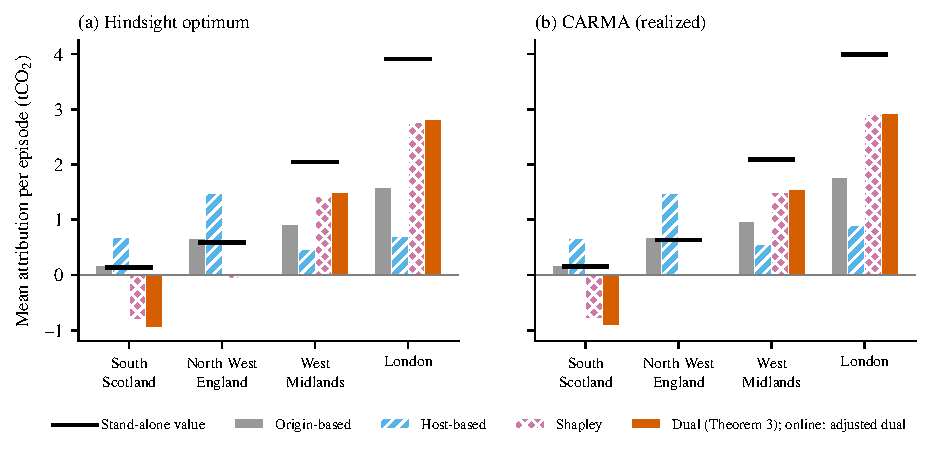
\includegraphics[width=\textwidth]{fig9_fairness.pdf}
\caption{Mean weekly carbon attribution by site under four rules, compared with each site's stand-alone value (black lines), 52 test weeks of 2024 at $\rho=0.5$. (a) Hindsight optimum. (b) CARMA's realized emissions. Negative values are net credits for contributing low-carbon capacity.}
\label{fig:fair}
\end{figure}


\section{Discussion}\label{sec:discussion}

\subsection{Managerial implications}

\paragraph{Protect scarce clean capacity} In multi-site carbon-aware scheduling, the largest operational loss does not come from imperfect carbon forecasts. It comes from spending low-carbon capacity on work that could have waited or run elsewhere. Proposition~\ref{prop:myopic} and Theorem~\ref{thm:lb} show this in the worst case, and the experiments confirm it on average. With migration allowed, a myopic planner with perfect carbon foresight is still 17--21\% above the optimum in the synthetic experiment and 34\% above it on the trace-derived workload. Clean capacity at a low-carbon site should be treated as a scarce resource with an opportunity cost, as in revenue management. A simple protection level (MPC-Protect) captures part of this value. CARMA captures more, because its ghost jobs price the protection hour by hour from the operator's own history. The result held when the profile underestimated demand by 28\% and demand was bursty. A stochastic lookahead over sampled demand scenarios does slightly better in Great Britain and the United States (0.4--1.0 points of gap) and is level with CARMA elsewhere, at 12--37 times the decision time; when the planning network can be solved in seconds, it is a reasonable alternative. The value of demand information is not specific to one grid: the advantage of CARMA over the best baseline without it is 7.3 points in Europe and 1.7--2.8 points in the other three fleets, and it tends to be smaller where the sites are closer to each other relative to their mean intensity.

\paragraph{Invest in forecasts where they pay} The value of better intensity forecasts depends on the rest of the policy. For a myopic multi-site planner, perfect forecasts are worth only 1.4--2.4 percentage points; once demand is anticipated they are worth 4--7 points; without migration they are worth almost the whole remaining gap. Persistent errors, such as a missed day-ahead wind front, are more costly than independent ones. Forecasting effort, for example the integration of numerical weather predictions~\cite{maji2022carboncast,lowry2018day}, should therefore target day-level biases, and in multi-site settings it should follow the fix of demand myopia.

\paragraph{Use risk premia with care} The conformal cost views help a myopic planner but not CARMA. They work by making volatile sites and distant hours look dirtier, which crudely imitates anticipation. Once demand is anticipated, the same distortion gives up useful deferrals. Calibrated quantiles are better suited to reporting and to service-level decisions than to reshaping costs by default.

\paragraph{Emissions or service near saturation} Without migration and at high load, every carbon-aware policy delayed work, and under a service-adjusted metric carbon-agnostic operation was preferable. Operators should combine temporal shifting with explicit service constraints, or restrict it, when local capacity is close to saturation.

\paragraph{Attributional versus physical savings} The headline reductions are attributional: they measure how much of the work runs where and when the \emph{average} regional mix is clean. Within a single market such as Great Britain, moving load between regions mostly reassigns the average mix. Under a stylized marginal-emission proxy, the achievable reduction fell from 58\% to 14\% and CARMA's advantage over MPC became small (0.6 points). Carbon-aware shifting is physically most valuable when it absorbs low-carbon output that would otherwise be curtailed, for example behind transmission constraints between Scotland and England, when temporal shifts change which plant is marginal, or when sites lie in different markets. Our marginal accounting is a stylized proxy, not an estimate of GB-wide abatement, so it indicates the direction and rough size of this effect rather than its value. In such settings a marginal signal should drive the scheduler. The scheduling framework is unchanged: only the cost coefficients of the flow network change. Idle power works in the same direction. If servers stay powered, deferral saves only their dynamic energy, and carbon-aware scheduling should be paired with right-sizing~\cite{lin2013dynamic}.

\paragraph{Fair internal carbon accounting} Pooling halved the hindsight emissions of the four sites. However, origin-based accounting, which charges each site for its own jobs wherever they run, would have made South Scotland worse off than on its own in every episode. A pool of organizations or business units allocated this way is unstable, because its cleanest members have an incentive to leave. The dual attribution of Theorem~\ref{thm:core} charges each site the carbon shadow price of its demand and credits it for the capacity it contributes. It is budget-balanced, no coalition would prefer to secede, and it is a by-product of the scheduling problem. It suits internal carbon pricing and the sharing of the benefits of carbon-aware scheduling among business units. It is not a substitute for external GHG Protocol reporting, where negative Scope~2 emissions do not exist~\cite{ghg2015scope2}. The players must also be entities that could credibly schedule on their own, such as separate operators, business units with their own capacity, or tenants with reserved shares. Because credits reward contributed capacity, capacity declarations should be audited.

\paragraph{Deployment} CARMA needs a carbon-intensity feed (average or marginal), a demand profile computed from the operator's own job logs and a network-flow solver. It decides within tens of milliseconds and returns a plan that is optimal for its model, which makes its decisions auditable. Absolute savings scale with the fleet: for the 1{,}700-server fleet simulated here, CARMA saves about 16~tCO$_2$ per year relative to myopic control and about 165~tCO$_2$ relative to carbon-agnostic operation, in attributional terms.

\subsection{Limitations and future research}

The study has several limitations. First, the synthetic workloads use a profile learned from the same generator, which favors anticipation. The trace experiment partly addresses this concern, but it covers only four evaluation days of one cluster, arrival times are first task starts, work is based on planned CPU requests, deadlines and origins are synthetic, and jobs are batched. Its 156 episodes vary carbon conditions but share one demand chronology. Second, the regional intensities published by NESO are modeled estimates, used here as realized values, 52 hours of them are missing and filled by persistence, and the marginal analysis relies on a stylized proxy with fixed thresholds, not on a dispatch model or observed curtailment. Third, the facility parameters (PUE, network energy, a 96-core server) are stylized, and embodied emissions are outside the scope except as the floor that makes $\theta$ finite. Fourth, the forecaster excludes weather inputs, so its day-ahead skill is limited. Fifth, bag-of-tasks jobs with free preemption and migration are an idealization: jobs with state, data gravity, bandwidth limits or data-sovereignty constraints would add restrictions that break the pure network structure. Sixth, the guarantees of Theorem~\ref{thm:carma} assume a backstop resource, a positive emission floor and an episode within the planning window, none of which holds in the simulations. The theorem describes the mechanism and the experiments its empirical profile. Its robustness term is shared by all on-time policies and is far from the $\Omega(\sqrt\theta)$ lower bound. Seventh, the core property is exact only for the hindsight benchmark, and the online adjustment is a heuristic. Eighth, Scenario-MPC was tuned and tested with a modest number of scenarios and was not included in the sensitivity analysis because of its cost. Ninth, the additional fleets use production-based lifecycle intensities computed from open generation data, uniform PUE and a capacity layout that mirrors the British one (tested against its reverse), and they cover Europe, the Americas and Oceania only: no open hourly generation data could be retrieved for Asia or Africa, and the New Zealand site is a single national grid.

Several extensions follow naturally. The ghost-demand profile could be replaced by probabilistic arrival forecasts, with the anticipation weight set by a newsvendor-type argument, or by scenario-based planning that treats demand and carbon uncertainty jointly~\cite{bertsimas2004price}. Tightening robustness toward the lower bound while retaining consistency, for example by protecting deferral decisions with reservation prices~\cite{elyaniv2001optimal,lechowicz2025learning}, is an open theoretical question. The framework can also be driven by marginal emission signals, coupled with right-sizing, on-site renewables and storage~\cite{souza2023ecovisor,acun2023carbon} and demand-response programs~\cite{wierman2014opportunities}, and evaluated across several electricity markets.

\section{Conclusions}\label{sec:conclusion}

We studied carbon-aware scheduling of deferrable computing workloads across data-center sites. The offline problem is a minimum-cost flow, which gives exact oracles (after quantization) and fast online planning. Uncertainty about demand alone forces every online algorithm to a competitive ratio of order $\sqrt\theta$, even with perfect carbon forecasts. CARMA, which adds ghost jobs for expected arrivals to the planning network, is deadline-safe under any predictions, optimal under exact predictions and linearly degrading in the prediction error when a backstop exists and episodes fit within the planning window. The dual prices of the pooled problem give a carbon attribution in the core of the hindsight pooling game.

In out-of-sample tests on five grids across four continents, CARMA came within 2.7--9.8\% of the clairvoyant optimum at a load of 0.5, against 4.4--16.3\% for the best baseline without demand information, and within 21.2\% on a trace-derived workload against 27.5\%. A scenario-based stochastic lookahead with the same demand information was level with CARMA or at most 1 point better, but 12--37 times slower. Anticipating demand was worth more than perfect carbon foresight, and correlated forecast errors hurt more than independent ones. Three results qualify these gains. Without migration, reductions are small and near saturation carbon-aware shifting can be worse than carbon-agnostic operation under a service-adjusted metric. Under a stylized marginal-emission proxy, CARMA's advantage over myopic control shrank to 0.6 points for Great Britain. Origin-based and host-based carbon accounting violated coalitional stability in every test week, whereas the dual attribution did so only for the heuristic online adjustment, and then rarely.

Asia and Africa are not covered, because no open hourly generation data could be retrieved. Carbon-aware computing is most effective when schedulers plan for the work that has not yet arrived, not only for the grid conditions that lie ahead, and when its benefits are measured and shared on a sound basis.


\section*{CRediT authorship contribution statement}
\textbf{Quang-Vinh Dang:} Conceptualization, Methodology, Software, Data curation, Formal analysis, Investigation, Validation, Visualization, Writing -- original draft, Writing -- review \& editing.

\section*{Declaration of competing interest}
The author declares no known competing financial interests or personal relationships that could have appeared to influence the work reported in this paper.

\section*{Funding}
This research did not receive any specific grant from funding agencies in the public, commercial, or not-for-profit sectors.

\section*{Data availability}
The carbon-intensity data are publicly available from the NESO Carbon Intensity API~\cite{nesoapi} under the CC BY 4.0 license. The generation-mix data of the additional grids are publicly available from Energy-Charts, the EIA-930 bulk files, the ONS open-data portal and the New Zealand Electricity Authority. The data snapshot used in this study, all code, the workload generator with fixed random seeds, and all raw experiment outputs are available from the author's repository (\url{https://github.com/vinhqdang/Sustainable-Operations-and-Computers}).

\appendix
\setcounter{figure}{0}\setcounter{table}{0}
\makeatletter\@addtoreset{figure}{section}\@addtoreset{table}{section}\makeatother
\renewcommand{\thefigure}{\Alph{section}.\arabic{figure}}
\renewcommand{\thetable}{\Alph{section}.\arabic{table}}
\section{Proofs}\label{app:proofs}

\paragraph{Atoms} Splitting a job $j$ into sub-jobs $j_1,\dots,j_k$ with work $w_{j_i}$ and widths $m_{j_i}=m_jw_{j_i}/w_j$ does not change the optimal value of any planning problem. Given a solution for the merged job, the allocation $x_{j_i s}(t)=x_{js}(t)\,w_{j_i}/w_j$ satisfies every constraint of the split problem at the same cost. Conversely, summing the sub-job allocations gives a feasible allocation for the merged job, because $\sum_i m_{j_i}=m_j$. Splitting also preserves window-feasibility, since $w_{j_i}/m_{j_i}=w_j/m_j$. We may therefore compare true and predicted job sets atom by atom.

\subsection{Proof of Theorem~\ref{thm:lb}}

Normalize $L=1$, so $U=\theta$. Site $A$ has one server with cost $p\in[1,\theta]$ in hour 0 and cost 1 in hour 1. Site $B$ has ample capacity at cost $\theta$ in both hours. Transfer costs are zero. A flexible job ($w=m=1$, window $\{0,1\}$) is released at $t=0$. The adversary either releases nothing more (scenario 1) or releases an urgent job ($w=m=1$, window $\{1\}$) at $t=1$ (scenario 2). All costs are known in advance.

Consider any deterministic online algorithm that may split work fractionally, and let $x\in[0,1]$ be the amount of flexible work it runs at $t=0$. Running at $B$ in hour 0 costs $\theta\ge p$ and is dominated, so we may assume this work runs at $A$. In scenario 1 the algorithm finishes the remaining $1-x$ at $A$ in hour 1, so $\mathrm{ALG}_1=xp+(1-x)$, while $\mathrm{OPT}_1=1$. In scenario 2, hour 1 must process $2-x$ units and $A$ can take only one of them, so $\mathrm{ALG}_2=xp+1+(1-x)\theta$, while $\mathrm{OPT}_2=p+1$. The ratio $r_1(x)=1+x(p-1)$ increases in $x$, and the ratio $r_2(x)=\big(1+\theta-x(\theta-p)\big)/(p+1)$ decreases in $x$. Hence $\min_x\max\{r_1,r_2\}$ is attained where they are equal, at $x^*=(\theta-p)/(p^2-p-1+\theta)\in[0,1]$, and its value is
\[
1+\frac{(p-1)(\theta-p)}{p^2-p-1+\theta}.
\]
The adversary chooses $p$ to maximize this value, which gives $R^*(\theta)$. The choice $p=\sqrt\theta$ gives the stated closed-form lower bound. For a randomized algorithm, the expected cost in each scenario is affine in $x$, so it equals the cost of the deterministic fractional algorithm that plays $\mathbb{E}[x]$, and the bound applies against an oblivious adversary. Myopic MPC sees only the flexible job at $t=0$ and, for any $p>1$, defers it entirely to the cheaper hour 1 ($x=0$). Its ratio in scenario 2 is $(1+\theta)/(p+1)$, which tends to $(1+\theta)/2$ as $p\to 1^+$, so its competitive ratio is at least $(1+\theta)/2$. \hfill$\square$

\subsection{Proof of Proposition~\ref{prop:robust} and Theorem~\ref{thm:carma}}

\paragraph{Proposition~\ref{prop:robust}} A policy that completes all work $W$ on time executes every server-hour at a unit cost of at most $U$, so its emissions are at most $UW$. Every server-hour in the oracle's solution costs at least $L$, and slack costs $\Pi>U\ge L$, so $\mathrm{OPT}\ge LW$. \hfill$\square$

\paragraph{Deadline safety} We first show by induction that every pending real job $j$ is window-feasible at the start of every hour: its remaining work satisfies $r_j\le m_j(d_j-t)$. This holds at release by (A1). Suppose it holds at hour $t$, and suppose the plan of CARMA leaves some real work $u_j>0$ unfinished. Because $r_j\le m_j(d_j-t)$, some hour $\tau\in[t,d_j)$ carries less than $m_j$ units of job $j$ in the plan. Moving a small amount of $u_j$ to the backstop in hour $\tau$ keeps the plan feasible, because the backstop has unlimited capacity. It changes the planned cost by a negative amount, because the planner prices the backstop at most at $U<\Pi$ (A1), whatever its forecasts of the other costs are. Since $d_j-t\le H$ (A1), hour $\tau$ lies inside the planning window. This contradicts optimality, so the plan completes all real work. After the first hour is executed, the rest of the plan is a feasible completion, so $r_j'\le m_j(d_j-t-1)$ and the induction step holds. No real job is ever late, whatever the ghost jobs are, and $\theta$-competitiveness follows from Proposition~\ref{prop:robust}.

\paragraph{Telescoping} Let $\sigma_t$ be the state at the start of hour $t$: the remaining work of all real jobs released by $t$. Let $V_t(\sigma,G;c)$ be the optimal value of (\ref{eq:obj})--(\ref{eq:cap}) over hours $t,\dots,T-1$ for the pending jobs $\sigma$ and the future jobs $G$ under costs $c$. Write $\bar V_t=V_t(\sigma_t,F_t;c)$, so that $\bar V_0=\mathrm{OPT}$ and $\bar V_T=0$. For a feasible hour-$t$ allocation $x$ with cost $g_t(x)$ and successor state $\sigma^+(x)$, define
\[
Q_t(x)=g_t(x)+V_{t+1}\big(\sigma^+(x),F_t;c\big),\qquad \hat Q_t(x)=g_t(x)+V_{t+1}\big(\sigma^+(x),\hat F_t;\hat c_t\big).
\]
By dynamic programming over a deterministic future, $\min_xQ_t(x)=\bar V_t$, and $Q_t(x_t)=g_t(x_t)+\bar V_{t+1}$ for the executed action $x_t$. Summing over $t$ gives
\[
\mathrm{ALG}-\mathrm{OPT}=\sum_{t=0}^{T-1}\delta_t,\qquad \delta_t=Q_t(x_t)-\min_xQ_t(x)\ge 0.
\]
Ghost jobs are released at $t+1$ or later, the planning window reaches $T$ by (A2), and hour-$t$ costs are observed. The planning problem solved by CARMA at hour $t$ is therefore exactly $\min_x\hat Q_t(x)$, and $x_t$ is a minimizer.

\paragraph{One-step loss} Let $x^*\in\arg\min Q_t$. Since $\hat Q_t(x_t)\le\hat Q_t(x^*)$, we have $\delta_t\le\Delta(x_t)-\Delta(x^*)$, where $\Delta=Q_t-\hat Q_t$. Write $\Delta=D_1+D_2$ with
\begin{align*}
D_1(x)&=V_{t+1}(\sigma^+(x),F_t;c)-V_{t+1}(\sigma^+(x),\hat F_t;c),\\
D_2(x)&=V_{t+1}(\sigma^+(x),\hat F_t;c)-V_{t+1}(\sigma^+(x),\hat F_t;\hat c_t).
\end{align*}
\emph{Cost error.} An optimal solution under $\hat c_t$ is feasible under $c$, and its cost changes by at most $\varepsilon_t$ per unit of flow on future-hour arcs. The same holds with the roles of $c$ and $\hat c_t$ exchanged. Hence $|D_2(x)|\le\varepsilon_tW_t$ for all $x$, and $D_2(x_t)-D_2(x^*)\le 2\varepsilon_tW_t$.

\emph{Demand error.} Under (A1), the penalty attached to a window-feasible job does not affect any optimal value, provided it is at least $U$. If a solution leaves slack on such a job, the argument used for robustness moves that slack to the backstop at no greater cost. True future jobs (penalty $\Pi$) and ghost jobs (penalty $\Pi_g$) can therefore be treated as identical atoms whenever they coincide. Let $a$ be a window-feasible atom and $G$ any set of future jobs. For every state $\sigma$,
\[
Lw_a\;\le\;V(\sigma,G\cup\{a\})-V(\sigma,G)\;\le\;Uw_a.
\]
For the upper bound, add $a$ to an optimal solution for $G$ by running it on the backstop at rate $w_a/(d_a-a_a)\le m_a$ in every hour of its window. For the lower bound, delete $a$'s flow and slack from an optimal solution for $G\cup\{a\}$; each deleted unit cost at least $\min\{L,\Pi_a\}=L$, since $\Pi_a\ge U\ge L$. Now transform $\hat F_t$ into $F_t$ by removing $\hat F_t\setminus F_t$ and adding $F_t\setminus\hat F_t$, one atom at a time. Then $D_1(x)$ is a sum of increments, each lying in $[Lw_a,Uw_a]$ (with a minus sign for removals) for every $x$. Therefore $D_1(x_t)-D_1(x^*)\le(U-L)\sum_aw_a=(U-L)\,d_t$.

Combining the two bounds gives $\delta_t\le(U-L)d_t+2\varepsilon_tW_t$. Summing over $t$ and taking the minimum with the robustness bound proves (\ref{eq:smooth}). If $d_t=\varepsilon_t=0$ for all $t$, then $\delta_t=0$ and $\mathrm{ALG}=\mathrm{OPT}$. \hfill$\square$

\subsection{Proof of Theorem~\ref{thm:core}}

Write the problem of coalition $C$ as $c(C)=\min\{c^\top z: A_{=}z=b_{=}(C),\ A_{\le}z\le b_{\le}(C),\ z\ge 0\}$, where $z=(x,u)$. Jobs submitted outside $C$ have zero work and zero width, and sites outside $C$ have zero capacity. This forces the corresponding flows to zero, so the problem coincides with the stand-alone problem of $C$. The right-hand side is additive over sites: $b(C)=\sum_{o\in C}b^o$, where $b^o$ collects the work and widths of the jobs submitted at $o$ and the capacity of site $o$. The matrix $A$ and the cost $c$ do not depend on $C$. The dual problem $\max\{b(C)^\top y: A^\top y\le c,\ y_{\le}\le 0\}$ therefore has a feasible set that is the same for all coalitions.

Let $y^*=(\lambda,\nu,\mu)$ be an optimal dual solution for $\mathcal S$. The slack variables make every primal problem feasible, and costs are non-negative, so strong duality gives $c(\mathcal S)=b(\mathcal S)^\top y^*=\sum_o(b^o)^\top y^*=\sum_o\phi_o$, which is budget balance. For any coalition $C$, $y^*$ is dual-feasible for $C$, so weak duality gives $c(C)\ge b(C)^\top y^*=\sum_{o\in C}\phi_o$, which is the core condition~\cite{owen1975core}. Expanding $(b^o)^\top y^*$ gives (\ref{eq:phi}). By Proposition~\ref{prop:flow} the problem is a min-cost flow, so optimal node potentials, together with the reduced costs they induce on saturated capacity arcs, also give an optimal dual solution. Any optimal dual solution can be used; in our experiments it is returned by the LP solver HiGHS. \hfill$\square$

\section{Forecast evaluation}\label{app:forecast}

Table~\ref{tab:forecast} and Fig.~\ref{fig:forecast}a summarize forecast accuracy in 2024; hours affected by gap filling are excluded. Averaged over horizons and sites, the direct GBM forecaster has a mean absolute error (MAE) of 31.7~gCO$_2$/kWh, against 35.3 for persistence and 40.9 for the seasonal-naive forecast. The advantage is largest at short and medium horizons: MAE falls by 23\% at 1 hour (6.4 against 8.3) and by 24\% at 6 hours (23.6 against 31.2). The advantage shrinks with the horizon, and at 24 hours the GBM is worse than both benchmarks (42.7 against 40.9). Without weather forecasts, day-ahead changes in wind output are hard to predict from the intensity history alone~\cite{maji2022carboncast}. By site, the improvement over persistence is largest in absolute terms for the volatile southern sites (West Midlands 50.2 against 57.7, London 38.0 against 43.4), although their MAE is also the highest. In South Scotland, where intensity is low and often flat, persistence is better overall (14.5 against 16.2). Diebold--Mariano tests~\cite{diebold1995comparing} with absolute-error loss and HAC variance confirm these patterns. For the three English sites, the GBM is significantly more accurate than persistence at horizons of 1--18 hours ($p\le0.002$) and indistinguishable at 24 hours ($p\ge0.09$). For South Scotland it is significantly better at 1 and 3 hours, indistinguishable at 6 hours and significantly worse from 12 hours onwards.

\begin{table}[!htbp]
\centering
\caption{Forecast accuracy on the 2024 test year (MAE in gCO$_2$/kWh; mean over sites unless stated).}
\label{tab:forecast}
\small
\begin{tabular}{lrrrrrrr}
\toprule
 & \multicolumn{5}{c}{Horizon $h$ (hours)} & \multicolumn{2}{c}{All horizons} \\
\cmidrule(lr){2-6}\cmidrule(lr){7-8}
Model & 1 & 3 & 6 & 12 & 24 & MAE & RMSE \\
\midrule
Persistence & 8.3 & 20.0 & 31.2 & 38.6 & \textbf{40.9} & 35.3 & 49.2 \\
Seasonal naive (24 h) & 40.9 & 40.9 & 40.8 & 40.8 & \textbf{40.9} & 40.9 & 57.4 \\
Direct GBM (this study) & \textbf{6.4} & \textbf{15.1} & \textbf{23.6} & \textbf{34.5} & 42.7 & \textbf{31.7} & \textbf{41.6} \\
\bottomrule
\end{tabular}

\smallskip
\parbox{0.92\textwidth}{\footnotesize MAE by site over all horizons (persistence / GBM): South Scotland 14.5 / 16.2; North West England 25.5 / 22.3; West Midlands 57.7 / 50.2; London 43.4 / 38.0.}
\end{table}

\begin{figure}[!htbp]
\centering
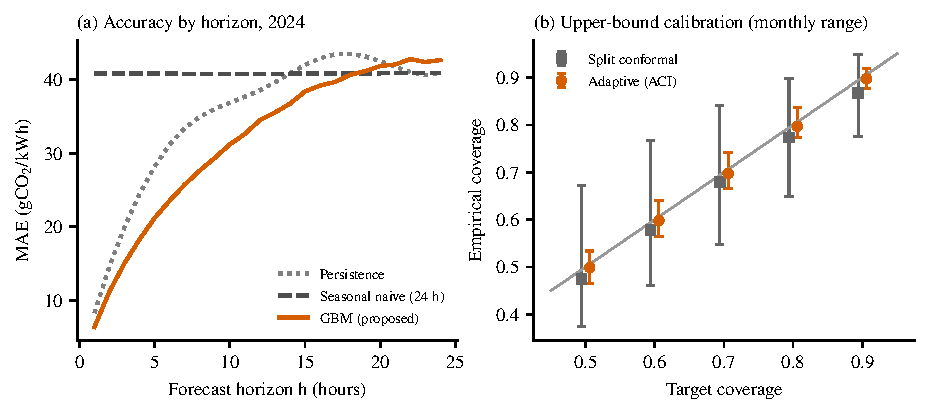
\includegraphics[width=\textwidth]{fig3_forecast.pdf}
\caption{Forecast evaluation in 2024. (a) MAE by horizon, averaged over sites. (b) Empirical coverage of one-sided upper bounds $U^\beta$ against the target level $\beta$ for static split conformal calibration and adaptive conformal inference (ACI). Markers show the annual coverage and bars the range across the 12 months.}
\label{fig:forecast}
\end{figure}

Calibration matters more than point accuracy for the risk-adjusted cost view, and Fig.~\ref{fig:forecast}b shows the effect of distribution shift. Static split-conformal bounds, calibrated on July--September 2023, under-cover in 2024 at every level: at $\beta=0.9$, annual coverage was 0.868 and monthly coverage ranged from 0.78 to 0.95. With the adaptive recalibration, annual coverage is within 0.003 of the target at all levels (0.499, 0.598, 0.697, 0.797 and 0.898). Monthly coverage stays within about four percentage points of the target (at most 4.2 points), and coverage is uniform across horizons. At $\beta=0.5$, the recalibrated median lies on average 10.3~gCO$_2$/kWh below the point forecast, which reflects the downward drift in intensity that the static model does not capture. Coverage is not the whole story. In pinball loss, the adaptive bounds improve on static calibration at levels 0.5--0.7 (15.01 against 15.16 at 0.5) but are worse at 0.8 and 0.9 (9.07 against 8.36 at 0.9). Delayed feedback explains much of this. The level for horizon $h$ is updated only when the outcome is observed, $h$ hours after issue, so a day of under-forecasts drives the level of long horizons toward 1 before any correction arrives. At $\beta=0.9$, 5.6\% of the 2024 bounds (0.5\% at $\beta=0.8$) were at the fallback ceiling, the training-period maximum of the site. These features, together with the finite ceiling and the quantile grid, are why we treat the procedure as an empirical recalibration and do not invoke the coverage guarantee of ACI~\cite{gibbs2021adaptive}. Annual coverage says nothing about conditional coverage in the site-hours that the optimizer selects.

\section{Numerical check of Theorem~\ref{thm:carma}}\label{app:thm2check}

The weekly experiments of Section~\ref{sec:results} violate the assumptions of Theorem~\ref{thm:carma}, so we check the theorem separately in episodes that satisfy them (script \texttt{verify\_theorem2.py}). Each episode is one day ($T=24=H$ hours) of the synthetic workload, with days starting at 26 test weeks, a backstop of unlimited capacity at the episode's largest unit cost $U$ (A1), window-feasible jobs, real-job penalty $\Pi=10^4>U$ and ghost penalty $\Pi_g=U$. Ghost jobs are the true future jobs, each omitted from the predictions with probability $q$ (demand error), and the carbon forecasts of future hours receive i.i.d.\ Gaussian noise of standard deviation $\sigma$~gCO$_2$/kWh (carbon error). For each episode, we compute the clairvoyant optimum OPT with the backstop, the emissions of CARMA, and the right-hand side of the smoothness bound (\ref{eq:smooth}) from the realized $d_t$, $\varepsilon_t$ and $W_t$. There are 26 episodes for each of 12 settings (two loads and six error settings).

\begin{table}[!htbp]
\centering
\caption{Numerical check of Theorem~\ref{thm:carma} in one-day episodes with a backstop. ALG/OPT: emissions of CARMA relative to the clairvoyant optimum (mean and maximum over 26 episodes). Bound: mean ratio of the right-hand side of (\ref{eq:smooth}) to OPT. The bound held in every episode, and no real work was late.}
\label{tab:thm2}
\small
\begin{tabular}{rrrrrr}
\toprule
Load $\rho$ & $q$ & $\sigma$ & Mean ALG/OPT & Max ALG/OPT & Bound / OPT \\
\midrule
0.5 & 0 & 0 & 1.000 & 1.000 & 1.0 \\
0.5 & 0 & 25 & 1.011 & 1.031 & 37.7 \\
0.5 & 0 & 100 & 1.061 & 1.257 & 139.6 \\
0.5 & 0.1 & 0 & 1.009 & 1.072 & 6.4 \\
0.5 & 0.3 & 0 & 1.066 & 1.365 & 17.9 \\
0.5 & 0.3 & 100 & 1.094 & 1.332 & 160.2 \\
0.9 & 0 & 0 & 1.000 & 1.000 & 1.0 \\
0.9 & 0 & 25 & 1.001 & 1.003 & 19.3 \\
0.9 & 0 & 100 & 1.004 & 1.015 & 69.3 \\
0.9 & 0.1 & 0 & 1.001 & 1.011 & 3.6 \\
0.9 & 0.3 & 0 & 1.010 & 1.112 & 9.1 \\
0.9 & 0.3 & 100 & 1.010 & 1.029 & 78.2 \\
\bottomrule
\end{tabular}
\end{table}

Three observations follow. With exact predictions, CARMA reproduces the optimum to within the 0.01 server-hour quantization of the flow solver (relative difference at most $2\times10^{-5}$), which is consistency. No real work was late in any of the 312 episodes, in line with deadline safety. The smoothness bound holds in every episode but is loose by one to two orders of magnitude when predictions are wrong, because each misprediction enters $d_t$ in every hour in which it is visible. The realized excess over the optimum is at most 37\%, so the bound is a qualitative statement that errors enter linearly, not a tight prediction.

\section{Results on other grids at all loads}\label{app:multigrid}

\begin{table}[!htbp]
\centering
\caption{Results on five grids at all loads (migration allowed; 52 test weeks of 2024). Gaps to the oracle (\%). Advantage: gap of the best baseline without demand information minus CARMA's gap, with a 95\% block-bootstrap CI (points). Late: CARMA's share of late work (\%).}
\label{tab:multigrid_loads}
\scriptsize\setlength{\tabcolsep}{2.5pt}
\begin{tabular}{lrrrrrrlrr}
\toprule
Fleet & $\rho$ & \makecell{Oracle\\red.} & MPC & \makecell{MPC-\\Prot.} & \makecell{MPC+\\conf.} & CARMA & \makecell{Best baseline} & \makecell{Advantage (CI)} & Late \\
\midrule
\inputtable{table_multigrid_loads.tex}
\bottomrule
\end{tabular}
\end{table}


\bibliographystyle{elsarticle-num}
\bibliography{references}

\end{document}
